\documentclass[a4paper, openany]{memoir}

\usepackage[utf8]{inputenc}
\usepackage[T1]{fontenc} 
\usepackage[english]{babel}

\usepackage{fancyhdr}
\usepackage{float}

\usepackage{amsmath}
\usepackage{amsthm}
\usepackage{amssymb}
\usepackage{enumitem}
\usepackage{multicol}
\usepackage[bookmarksopen=true,bookmarksopenlevel=2]{hyperref}
\usepackage{tikz}
\usepackage{listings}
\usepackage{xcolor}
\usepackage{indentfirst}
% \usepackage{graphicx}

\pagestyle{fancy}
\fancyhf{}
\fancyhead[LE]{\leftmark}
\fancyhead[RO]{\rightmark}
\fancyhead[RE, LO]{Algorithmics I}
\fancyfoot[LE, RO]{\thepage}
\fancyfoot[RE, LO]{Pete Gautam}

\usetikzlibrary{shapes, positioning}
\definecolor{codegreen}{rgb}{0,0.6,0}
\definecolor{codegray}{rgb}{0.5,0.5,0.5}
\definecolor{codepurple}{rgb}{0.58,0,0.82}
\definecolor{backcolour}{rgb}{0.95,0.95,0.92}

\lstdefinestyle{thestyle}{
    backgroundcolor=\color{backcolour},
    basicstyle=\ttfamily\footnotesize,
    keywordstyle=\color{red!80}\bfseries,
    ndkeywordstyle=\color{blue!80}\bfseries,
    identifierstyle=\color{black},
    commentstyle=\color{codegreen},
    stringstyle=\color{codepurple},
    breakatwhitespace=false,
    breaklines=true,
    captionpos=b,
    keepspaces=true,
    numberstyle=\tiny\color{codegray},
    numbers=left,
    numbersep=2pt,
    showspaces=false,
    showstringspaces=false,
    showtabs=false,          
    tabsize=2
}

\lstdefinelanguage{pseudocode}{ 
    keywords={new, return, this, null, if, in, while, else, for, get, set, class, and, or, not, min},
    ndkeywords={int, bool, List, Map, String, Node, Queue, Set, Vertex, Graph, Edge, void, true, false},
    sensitive=true,
    comment=[l]{//},
    morecomment=[s]{/*}{*/},
    morestring=[b]',
    morestring=[b]"
}

\lstset{style=thestyle}


\chapterstyle{thatcher}

\setcounter{chapter}{2}

\begin{document}

\chapter{Graph and Graph Algorithms}
\section{Introduction to Graphs}
\subsection{Undirected graphs}
An \emph{undirected graph} $G$ is defined to be the tuple $(V, E)$, where $V$ is a finite set of vertices (the vertex set), and $E$ is the set of edges, where every edge is a subset of $V$ of size 2. Pictorially, we can represent each vertex as a point and an edge as a line connecting two points. For example, if $V = \{a, b, c, x, y, z\}$ and $E = \{\{a, x\}, \{a, y\}, \{a, z\}, \{b, x\}, \{b, y\}, \{b, z\}, \{c, x\}, \{c, y\}, \{c, z\}\}$, then it can be represented as the following graph:
\begin{figure}[H]
    \centering
    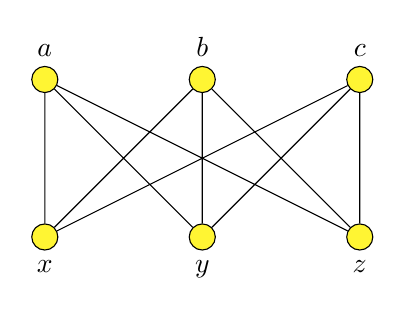
\begin{tikzpicture}
        \node[circle, draw, fill=yellow!80, label={90:$a$}] at (0, 0) (a) {};
        \node[circle, draw, fill=yellow!80, label={90:$b$}] at (2, 0) (b) {};
        \node[circle, draw, fill=yellow!80, label={90:$c$}] at (4, 0) (c) {};
        \node[circle, draw, fill=yellow!80, label={-90:$x$}] at (0, -2) (x) {};
        \node[circle, draw, fill=yellow!80, label={-90:$y$}] at (2, -2) (y) {};
        \node[circle, draw, fill=yellow!80, label={-90:$z$}] at (4, -2) (z) {};
        
        \draw (a) to (x)
        (a) to (y)
        (a) to (z)
        (b) to (x)
        (b) to (y)
        (b) to (z)
        (c) to (x)
        (c) to (y)
        (c) to (z);
    \end{tikzpicture}
    \caption{An undirected graph}
\end{figure}
\noindent A graph can have multiple pictorial representations. For example, the graph above can also be represented as the following graph:
\begin{figure}[H]
    \centering
    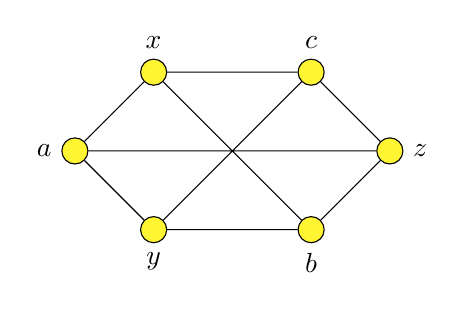
\begin{tikzpicture}
        \node[circle, draw, fill=yellow!80, label={90:$x$}] at (-1, 0) (x) {};
        \node[circle, draw, fill=yellow!80, label={90:$c$}] at (1, 0) (c) {};
        
        \node[circle, draw, fill=yellow!80, label={180:$a$}] at (-2, -1) (a) {};
        \node[circle, draw, fill=yellow!80, label={0:$z$}] at (2, -1) (z) {};
        
        \node[circle, draw, fill=yellow!80, label={-90:$y$}] at (-1, -2) (y) {};
        \node[circle, draw, fill=yellow!80, label={-90:$b$}] at (1, -2) (b) {};
        
        \draw (a) to (x)
            (a) to (y)
            (a) to (z)
            (b) to (x)
            (b) to (y)
            (b) to (z)
            (c) to (x)
            (c) to (y)
            (c) to (z);
    \end{tikzpicture}
    \caption{Another representation of the undirected graph above}
\end{figure}
We say two vertices are \emph{adjacent} if there is an edge between them. Otherwise, the two vertices are \emph{non-adjacent}. For example, in the graph above, vertices $a$ and $z$ are adjacent. We say a vertex is \emph{incident} of an edge if it is part of the edge. A \emph{path} traverses through edges and goes from one vertex to another. Its length is the number of edges present. For example, $a \to x \to b \to y \to c$ is a path of length 4. A \emph{cycle} is a path that starts and ends at the same node. For example, $a \to x \to b \to y \to a$ is a cycle of length 4. The \emph{degree} of a vertex is the number of edges it is incident to. For example, all the vertices above have degree 3.

A graph is \emph{connected} if there is a path between every pair of vertices. For example, the following is a connected graph.
\begin{figure}[H]
    \centering
    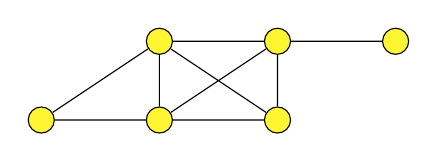
\begin{tikzpicture}
        \node[circle, draw, fill=yellow!80] (u) at (0, 0) {};
        \node[circle, draw, fill=yellow!80] (v) at (1.5, 0) {};
        \node[circle, draw, fill=yellow!80] (w) at (3, 0) {};
        \node[circle, draw, fill=yellow!80] (x) at (1.5, 1) {};
        \node[circle, draw, fill=yellow!80] (y) at (3, 1) {};
        \node[circle, draw, fill=yellow!80] (z) at (4.5, 1) {};
        
        \draw (u) to (x)
            (u) to (v)
            (v) to (w)
            (x) to (y)
            (x) to (v)
            (x) to (w)
            (y) to (w)
            (v) to (y)
            (y) to (z);
    \end{tikzpicture}
    \caption{A connected graph}
\end{figure}
\noindent If a graph is not connected, it is composed of two or more connected components, like in the case below.
\begin{figure}[H]
    \centering
    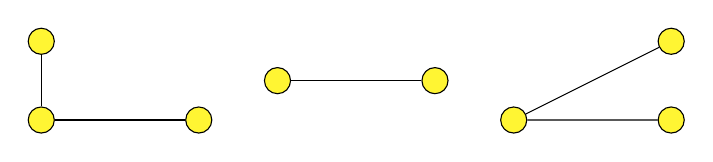
\begin{tikzpicture}
        \node[circle, draw, fill=yellow!80] (a1) at (0, 0) {};
        \node[circle, draw, fill=yellow!80] (a2) at (2, 0) {};
        \node[circle, draw, fill=yellow!80] (a3) at (0, 1) {};
        
        \draw (a1) -- (a2)
            (a1) -- (a3);
        
        \node[circle, draw, fill=yellow!80] (b1) at (3, .5) {};
        \node[circle, draw, fill=yellow!80] (b2) at (5, .5) {};
        
        \draw (b1) -- (b2);
        
        \node[circle, draw, fill=yellow!80] (c1) at (6, 0) {};
        \node[circle, draw, fill=yellow!80] (c2) at (8, 0) {};
        \node[circle, draw, fill=yellow!80] (c3) at (8, 1) {};
        
        \draw (c1) -- (c2)
            (c1) -- (c3);
    \end{tikzpicture}
    \caption{An unconnected graph with connected components}
    \label{fig:unconnected_forest}
\end{figure}
\noindent A graph is a \emph{tree} if it is connected and doesn't have any cycles. For example, the following is a tree.
\begin{figure}[H]
    \centering
    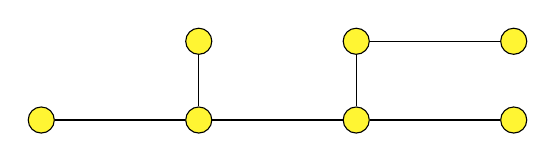
\begin{tikzpicture}
        \node[circle, draw, fill=yellow!80] (a) at (0, 0) {};
        \node[circle, draw, fill=yellow!80] (b) at (2, 0) {};
        \node[circle, draw, fill=yellow!80] (c) at (4, 0) {};
        \node[circle, draw, fill=yellow!80] (d) at (6, 0) {};
        \node[circle, draw, fill=yellow!80] (e) at (2, 1) {};
        \node[circle, draw, fill=yellow!80] (f) at (4, 1) {};
        \node[circle, draw, fill=yellow!80] (g) at (6, 1) {};
        
        \draw (a) -- (b)
            (b) -- (c)
            (c) -- (d)
            (b) -- (e)
            (c) -- (f)
            (f) -- (g);
    \end{tikzpicture}
    \caption{A Tree}
\end{figure}
A tree with $n$ vertices has precisely $n-1$ edges. Since it is connected, we must have at least $n-1$ edges (since we can reach from one vertex to another). Also, since it is not cyclic, we must have at most $n-1$ edges (if we have another edge, then we must have a vertex in at least two edges, and since it is connected, we can find a cycle from that vertex to itself).

A graph is a \emph{forest} if it is not cyclic and all its components are trees. For example, Figure \ref{fig:unconnected_forest} is a forest. A graph is \emph{complete} (or \emph{clique}) if every pair of vertices is joined by an edge. For example, the figure below is a clique on 4 vertices. 
\begin{figure}[H]
    \centering
    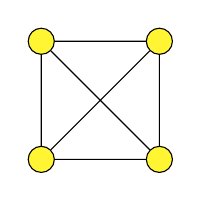
\begin{tikzpicture}
        \node[circle, draw, fill=yellow!80] at (0, 0) (a) {};
        \node[circle, draw, fill=yellow!80] at (0, 1.5) (b) {};
        \node[circle, draw, fill=yellow!80] at (1.5, 1.5) (c) {};
        \node[circle, draw, fill=yellow!80] at (1.5, 0) (d) {};
        
        \draw (a) to (b)
            (a) to (c)
            (a) to (d)
            (b) to (c)
            (b) to (d)
            (c) to (d);
    \end{tikzpicture}
    \caption{The clique on 4 vertices $K_4$}
\end{figure}
A graph is \emph{bipartile} if we can partition the vertices into two distinct sets $U$ and $W$ such that every edge joins a vertex in $U$ to a vertex in $W$. For example, the following is a partition of a complete bipartile graph on 6 vertices.
\begin{figure}[H]
    \centering
    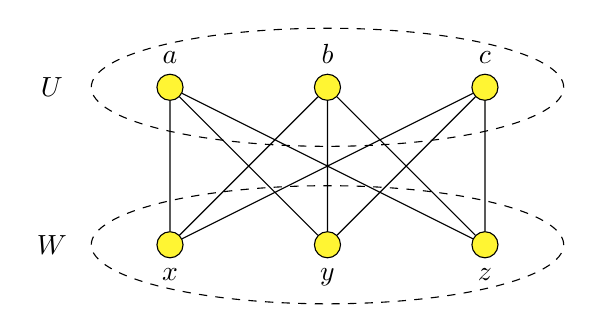
\begin{tikzpicture}
        \node[circle, draw, fill=yellow!80, label={90:$a$}] at (0, 0) (a) {};
        \node[circle, draw, fill=yellow!80, label={90:$b$}] at (2, 0) (b) {};
        \node[circle, draw, fill=yellow!80, label={90:$c$}] at (4, 0) (c) {};
        \node[circle, draw, fill=yellow!80, label={-90:$x$}] at (0, -2) (x) {};
        \node[circle, draw, fill=yellow!80, label={-90:$y$}] at (2, -2) (y) {};
        \node[circle, draw, fill=yellow!80, label={-90:$z$}] at (4, -2) (z) {};
        
        \draw (a) to (x)
            (a) to (y)
            (a) to (z)
            (b) to (x)
            (b) to (y)
            (b) to (z)
            (c) to (x)
            (c) to (y)
            (c) to (z);
            
        \draw[dashed] (2, -2) ellipse (3 and .75); 
        \draw[dashed] (2, 0) ellipse (3 and .75); 
        \node at (-1.5, -2) {$W$};
        \node at (-1.5, 0) {$U$};
    \end{tikzpicture}
    \caption{A complete bipartile graph $K_{3, 3}$}
\end{figure}
\noindent Bipartile graphs do not need to be complete, but the one above is. For instance, the following is an incomplete bipartile graph on 6 vertices.
\begin{figure}[H]
    \centering
    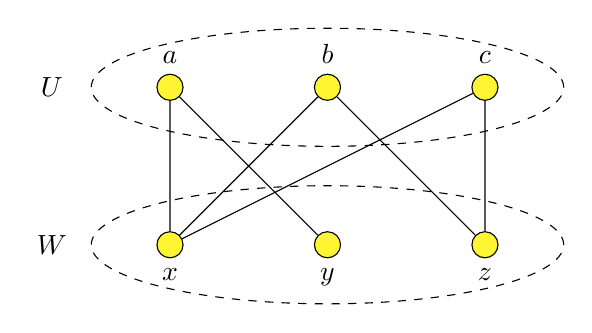
\begin{tikzpicture}
        \node[circle, draw, fill=yellow!80, label={90:$a$}] at (0, 0) (a) {};
        \node[circle, draw, fill=yellow!80, label={90:$b$}] at (2, 0) (b) {};
        \node[circle, draw, fill=yellow!80, label={90:$c$}] at (4, 0) (c) {};
        \node[circle, draw, fill=yellow!80, label={-90:$x$}] at (0, -2) (x) {};
        \node[circle, draw, fill=yellow!80, label={-90:$y$}] at (2, -2) (y) {};
        \node[circle, draw, fill=yellow!80, label={-90:$z$}] at (4, -2) (z) {};
        
        \draw (a) to (x)
            (a) to (y)
            (b) to (x)
            (b) to (z)
            (c) to (x)
            (c) to (z);
            
        \draw[dashed] (2, -2) ellipse (3 and .75); 
        \draw[dashed] (2, 0) ellipse (3 and .75); 
        \node at (-1.5, -2) {$W$};
        \node at (-1.5, 0) {$U$};
    \end{tikzpicture}
    \caption{An incomplete bipartile graph}
\end{figure}

\subsection{Directed graphs}
A \emph{directed graph} is like undirected graphs, but the edges have a direction. So, we have a finite set of vertices $V$ and a finite set of edges $E$, but every edge is an ordered pair $(x, y)$ of vertices. This corresponds to having an edge from $x$ to $y$. 

An example of a directed graph is given below.
\begin{figure}[H]
    \centering
    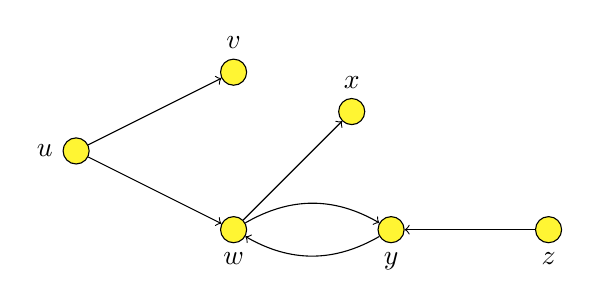
\begin{tikzpicture}
        \node[circle, draw, fill=yellow!80, label={180:$u$}] (u) at (0, 0) {};
        \node[circle, draw, fill=yellow!80, label={90:$v$}] (v) at (2, 1) {};
        \node[circle, draw, fill=yellow!80, label={-90:$w$}] (w) at (2, -1) {};
        \node[circle, draw, fill=yellow!80, label={90:$x$}] (x) at (3.5, .5) {};
        \node[circle, draw, fill=yellow!80, label={-90:$y$}] (y) at (4, -1) {};
        \node[circle, draw, fill=yellow!80, label={-90:$z$}] (z) at (6, -1) {};
        
        \draw[->] (u) to (v);
        \draw[->] (u) to (w);
        \draw[->] (w) to (x);
        \draw[->] (w) edge[bend left, below] (y)
            (y) edge[bend left, above] (w)
            (z) to (y);
    \end{tikzpicture}
    \caption{A directed graph}
\end{figure}
The terminology for directed graphs is slightly different to the ones we discussed above. In the particular case of the directed graph above, we say that:
\begin{itemize}
    \item the vertex $u$ is \emph{adjacent to} $v$, and the vertex $v$ is \emph{adjacent from} $u$;
    \item the vertex $y$ has \emph{in-degree} 2 and \emph{out-degree} 1;
    \item $u \to w \to x$ is a valid \emph{path}, but $x \to w \to u$ is not a path;
    \item $w \to y \to w$ is a valid \emph{cycle}.
\end{itemize}
\newpage

\section{Graph representations}
We can represent an undirected graph using an \emph{adjacency matrix}. This matrix contains one row and one column for each vertex. The value of row $i$ and column $j$ is a 1 if the $i$-th and the $j$-th vertices are adjacent; otherwise, the value is 0. We can also represent them as \emph{adjacency lists}. We store a list for each vertex. The list $i$ contains an entry for $j$ if the vertices $i$ and $j$ are adjacent.

For example, consider the undirected graph below.
\begin{figure}[H]
    \centering
    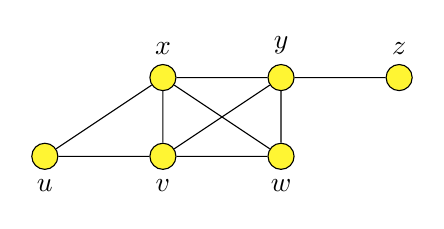
\begin{tikzpicture}
        \node[circle, draw, fill=yellow!80, label={-90:$u$}] (u) at (0, 0) {};
        \node[circle, draw, fill=yellow!80, label={-90:$v$}] (v) at (1.5, 0) {};
        \node[circle, draw, fill=yellow!80, label={-90:$w$}] (w) at (3, 0) {};
        \node[circle, draw, fill=yellow!80, label={90:$x$}] (x) at (1.5, 1) {};
        \node[circle, draw, fill=yellow!80, label={90:$y$}] (y) at (3, 1) {};
        \node[circle, draw, fill=yellow!80, label={90:$z$}] (z) at (4.5, 1) {};
        
        \draw (u) to (x)
            (u) to (v)
            (v) to (w)
            (x) to (y)
            (x) to (v)
            (x) to (w)
            (y) to (w)
            (v) to (y)
            (y) to (z);
    \end{tikzpicture}
    \caption{An undirected graph}
\end{figure}
\noindent We can represent it as the following adjacency matrix.
\begin{table}[H]
    \centering
    \begin{tabular}{c|cccccc}
         & $u$ & $v$ & $w$ & $x$ & $y$ & $z$ \\
        \hline
        $u$ & 0 & 1 & 0 & 1 & 0 & 0 \\
        $v$ & 1 & 0 & 1 & 1 & 1 & 0 \\
        $w$ & 0 & 1 & 0 & 1 & 1 & 0 \\
        $x$ & 1 & 1 & 1 & 0 & 1 & 0 \\
        $y$ & 0 & 1 & 1 & 1 & 0 & 1 \\
        $z$ & 0 & 0 & 0 & 0 & 1 & 0
    \end{tabular}
    \caption{The adjacency matrix representation for the undirected graph above}
\end{table}
\noindent Also, we can represent it as the following adjacency list.
\begin{table}[H]
    \centering
    \begin{tabular}{c|l}
        $u$ & $[v, x]$ \\
        $v$ & $[u, w, x, y]$ \\
        $w$ & $[v, x, y]$ \\
        $x$ & $[u, v, w, y]$ \\
        $y$ & $[v, w, x, z]$ \\
        $z$ & $[y]$
    \end{tabular}
    \caption{The adjacency list representation for the undirected graph above}
\end{table}
In the case of directed graphs, we can still use both adjacency matrices and adjacency lists. However, in an adjacency matrix, the entry in row $i$ and column $j$ is a 1 if there is an edge from $i$ to $j$; it is 0 otherwise. In an adjacency list, the list for vertex $i$ contains a vertex $j$ if there is an edge from $i$ to $j$.

For example, consider the directed graph below.
\begin{figure}[H]
    \centering
    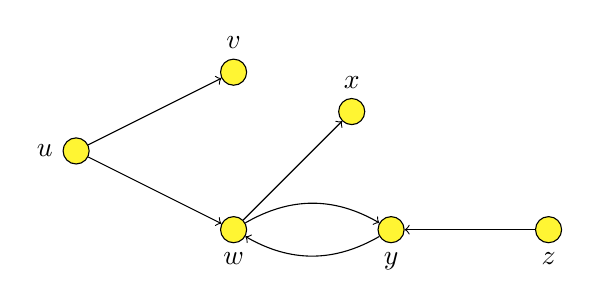
\begin{tikzpicture}
        \node[circle, draw, fill=yellow!80, label={180:$u$}] (u) at (0, 0) {};
        \node[circle, draw, fill=yellow!80, label={90:$v$}] (v) at (2, 1) {};
        \node[circle, draw, fill=yellow!80, label={-90:$w$}] (w) at (2, -1) {};
        \node[circle, draw, fill=yellow!80, label={90:$x$}] (x) at (3.5, .5) {};
        \node[circle, draw, fill=yellow!80, label={-90:$y$}] (y) at (4, -1) {};
        \node[circle, draw, fill=yellow!80, label={-90:$z$}] (z) at (6, -1) {};
        
        \draw[->] (u) to (v);
        \draw[->] (u) to (w);
        \draw[->] (w) to (x);
        \draw[->] (w) edge[bend left, below] (y)
            (y) edge[bend left, above] (w)
            (z) to (y);
    \end{tikzpicture}
    \caption{A directed graph}
\end{figure}
\noindent We can represent it as the following adjacency matrix.
\begin{table}[H]
    \centering
    \begin{tabular}{c|cccccc}
         & $u$ & $v$ & $w$ & $x$ & $y$ & $z$ \\
        \hline
        $u$ & 0 & 1 & 1 & 0 & 0 & 0 \\
        $v$ & 0 & 0 & 0 & 0 & 0 & 0 \\
        $w$ & 0 & 0 & 0 & 1 & 1 & 0 \\
        $x$ & 0 & 0 & 0 & 0 & 0 & 0 \\
        $y$ & 0 & 0 & 1 & 0 & 0 & 0 \\
        $z$ & 0 & 0 & 0 & 0 & 1 & 0
    \end{tabular}
    \caption{The adjacency matrix representation for the directed graph above}
\end{table}
\noindent Also, we can represent it as the following adjacency list.
\begin{table}[H]
    \centering
    \begin{tabular}{c|l}
        $u$ & $[v, w]$ \\
        $v$ & \\
        $w$ & $[ x, y]$ \\
        $x$ & \\
        $y$ & $[w]$ \\
        $z$ & $[y]$
    \end{tabular}
    \caption{The adjacency list representation for the directed graph above}
\end{table}
In the case of an undirected graph, the adjacency list features an edge $\{a, b\}$ twice- once as going from $a$ to $b$, and another time as going from $b$ to $a$. On the other hand, in the case of a directed graph, the adjacency list features an edge $(a, b)$ precisely once- it is only present in the list corresponding to the vertex $a$. In both cases, an adjacency matrix is an $|V| \times |V|$ array, while an adjacency list contains $|V|$ arrays which are themselves arrays containing vertices.

To implement this, we define classes for the entries of the adjacency lists, the vertices (as a linked list representation), and graphs (which includes the size of the graph and an array of vertices). The array allows for efficient access using the index of a vertex- we can then access it in constant time.

% The pseudocode for adjacency list implementation of a graph is given below.
% \lstinputlisting[language=pseudocode]{src/adjacencyList.psc}
\newpage

\section{Graph search and traversal}
Graph search and traversal is a systematic way to explore a graph, starting from some vertex. A search visits all the vertices by travelling along the edges. So, the traversal is efficient if it explores the graph in $O(|V| + |E|)$ time.

\subsection{Depth First Search}
Depth first search starts at a particular vertex, follows an edge from this vertex and continues on following some edge from that vertex until there is no edge to follow. It then backtracks and tries to take a different edge to find unvisited vertex until there are no more edges. Then, it starts the procedure all over again on an unvisited vertex (if the graph is not connected).

We illustrate this with an example below. So, consider the following graph with the starting vertex $e$.
\begin{figure}[H]
    \centering
    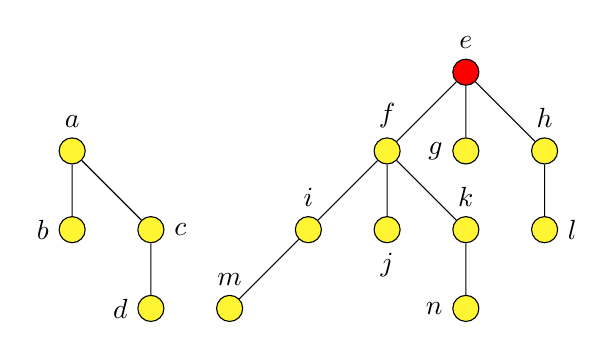
\begin{tikzpicture}
        \node[circle, draw, fill=yellow!80, label={90:$a$}] (a) at (0, 0) {};
        \node[circle, draw, fill=yellow!80, label={180:$b$}] (b) at (0, -1) {};
        \node[circle, draw, fill=yellow!80, label={0:$c$}] (c) at (1, -1) {};
        \node[circle, draw, fill=yellow!80, label={180:$d$}] (d) at (1, -2) {};
        
        \draw (a) to (b)
            (a) to (c)
            (c) to (d);
        
        \node[circle, draw, fill=red, label={90:$e$}] (e) at (5, 1) {};
        \node[circle, draw, fill=yellow!80, label={90:$f$}] (f) at (4, 0) {};
        \node[circle, draw, fill=yellow!80, label={180:$g$}] (g) at (5, 0) {};
        \node[circle, draw, fill=yellow!80, label={90:$h$}] (h) at (6, 0) {};
        \node[circle, draw, fill=yellow!80, label={90:$i$}] (i) at (3, -1) {};
        \node[circle, draw, fill=yellow!80, label={-90:$j$}] (j) at (4, -1) {};
        \node[circle, draw, fill=yellow!80, label={90:$k$}] (k) at (5, -1) {};
        \node[circle, draw, fill=yellow!80, label={0:$l$}] (l) at (6, -1) {};
        \node[circle, draw, fill=yellow!80, label={90:$m$}] (m) at (2, -2) {};
        \node[circle, draw, fill=yellow!80, label={180:$n$}] (n) at (5, -2) {};
        
        \draw (e) to (f)
            (e) to (g)
            (e) to (h)
            (f) to (i)
            (f) to (j)
            (f) to (k)
            (h) to (l)
            (i) to (m)
            (k) to (n);
    \end{tikzpicture}
    \caption{An undirected graph to be traversed via depth-first search.}
\end{figure}
\noindent We will label visited vertices in red. We the edge from $e$ and discover the vertex $f$.
\begin{figure}[H]
    \centering
    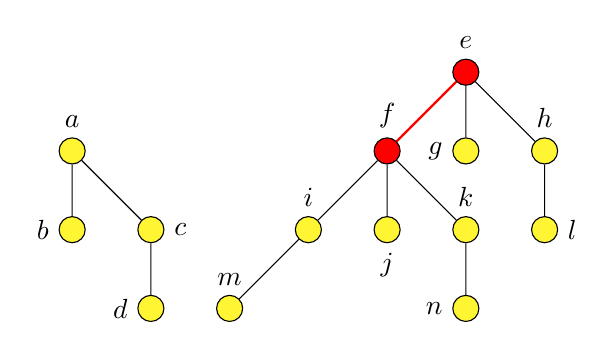
\begin{tikzpicture}
        \node[circle, draw, fill=yellow!80, label={90:$a$}] (a) at (0, 0) {};
        \node[circle, draw, fill=yellow!80, label={180:$b$}] (b) at (0, -1) {};
        \node[circle, draw, fill=yellow!80, label={0:$c$}] (c) at (1, -1) {};
        \node[circle, draw, fill=yellow!80, label={180:$d$}] (d) at (1, -2) {};
        
        \draw (a) to (b)
            (a) to (c)
            (c) to (d);
        
        \node[circle, draw, fill=red, label={90:$e$}] (e) at (5, 1) {};
        \node[circle, draw, fill=red, label={90:$f$}] (f) at (4, 0) {};
        \node[circle, draw, fill=yellow!80, label={180:$g$}] (g) at (5, 0) {};
        \node[circle, draw, fill=yellow!80, label={90:$h$}] (h) at (6, 0) {};
        \node[circle, draw, fill=yellow!80, label={90:$i$}] (i) at (3, -1) {};
        \node[circle, draw, fill=yellow!80, label={-90:$j$}] (j) at (4, -1) {};
        \node[circle, draw, fill=yellow!80, label={90:$k$}] (k) at (5, -1) {};
        \node[circle, draw, fill=yellow!80, label={0:$l$}] (l) at (6, -1) {};
        \node[circle, draw, fill=yellow!80, label={90:$m$}] (m) at (2, -2) {};
        \node[circle, draw, fill=yellow!80, label={180:$n$}] (n) at (5, -2) {};
        
        \draw[red, thick] (e) to (f);
        \draw (e) to (g)
            (e) to (h)
            (f) to (i)
            (f) to (j)
            (f) to (k)
            (h) to (l)
            (i) to (m)
            (k) to (n);
    \end{tikzpicture}
\end{figure}
\noindent The edge we just took is in red. At this point, we have two visited vertices- $e$ and $f$. The vertex $f$ is the current vertex. We take another edge from this vertex and discover the vertex $i$.
\begin{figure}[H]
    \centering
    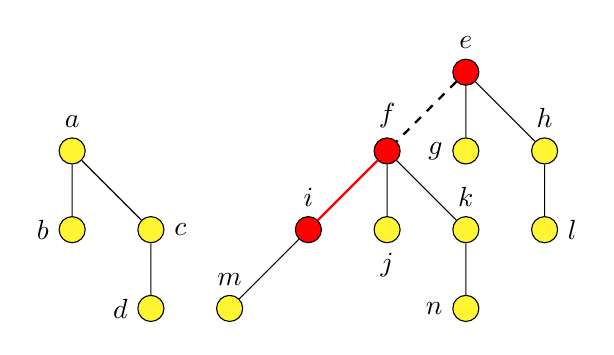
\begin{tikzpicture}
        \node[circle, draw, fill=yellow!80, label={90:$a$}] (a) at (0, 0) {};
        \node[circle, draw, fill=yellow!80, label={180:$b$}] (b) at (0, -1) {};
        \node[circle, draw, fill=yellow!80, label={0:$c$}] (c) at (1, -1) {};
        \node[circle, draw, fill=yellow!80, label={180:$d$}] (d) at (1, -2) {};
        
        \draw (a) to (b)
            (a) to (c)
            (c) to (d);
        
        \node[circle, draw, fill=red, label={90:$e$}] (e) at (5, 1) {};
        \node[circle, draw, fill=red, label={90:$f$}] (f) at (4, 0) {};
        \node[circle, draw, fill=yellow!80, label={180:$g$}] (g) at (5, 0) {};
        \node[circle, draw, fill=yellow!80, label={90:$h$}] (h) at (6, 0) {};
        \node[circle, draw, fill=red, label={90:$i$}] (i) at (3, -1) {};
        \node[circle, draw, fill=yellow!80, label={-90:$j$}] (j) at (4, -1) {};
        \node[circle, draw, fill=yellow!80, label={90:$k$}] (k) at (5, -1) {};
        \node[circle, draw, fill=yellow!80, label={0:$l$}] (l) at (6, -1) {};
        \node[circle, draw, fill=yellow!80, label={90:$m$}] (m) at (2, -2) {};
        \node[circle, draw, fill=yellow!80, label={180:$n$}] (n) at (5, -2) {};

        \draw[thick, dashed] (e) to (f);
        \draw[thick, red] (f) to (i);
        \draw (e) to (g)
            (e) to (h)
            (f) to (j)
            (f) to (k)
            (h) to (l)
            (i) to (m)
            (k) to (n);
    \end{tikzpicture}
\end{figure}
\noindent The visited edges are dashed. We have now visited three vertices- $e$, $f$ and $i$. There is only one edge from $i$ that we can take there, so we take it and visit $m$.
\begin{figure}[H]
    \centering
    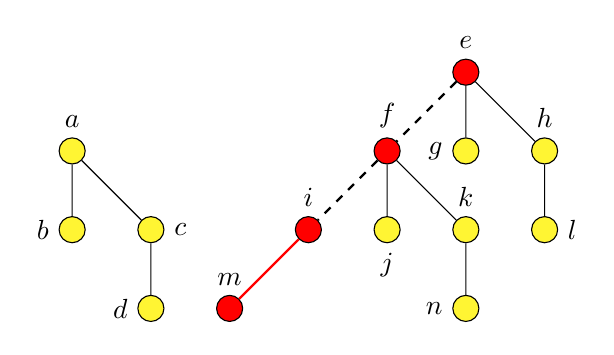
\begin{tikzpicture}
        \node[circle, draw, fill=yellow!80, label={90:$a$}] (a) at (0, 0) {};
        \node[circle, draw, fill=yellow!80, label={180:$b$}] (b) at (0, -1) {};
        \node[circle, draw, fill=yellow!80, label={0:$c$}] (c) at (1, -1) {};
        \node[circle, draw, fill=yellow!80, label={180:$d$}] (d) at (1, -2) {};
        
        \draw (a) to (b)
            (a) to (c)
            (c) to (d);
        
        \node[circle, draw, fill=red, label={90:$e$}] (e) at (5, 1) {};
        \node[circle, draw, fill=red, label={90:$f$}] (f) at (4, 0) {};
        \node[circle, draw, fill=yellow!80, label={180:$g$}] (g) at (5, 0) {};
        \node[circle, draw, fill=yellow!80, label={90:$h$}] (h) at (6, 0) {};
        \node[circle, draw, fill=red, label={90:$i$}] (i) at (3, -1) {};
        \node[circle, draw, fill=yellow!80, label={-90:$j$}] (j) at (4, -1) {};
        \node[circle, draw, fill=yellow!80, label={90:$k$}] (k) at (5, -1) {};
        \node[circle, draw, fill=yellow!80, label={0:$l$}] (l) at (6, -1) {};
        \node[circle, draw, fill=red, label={90:$m$}] (m) at (2, -2) {};
        \node[circle, draw, fill=yellow!80, label={180:$n$}] (n) at (5, -2) {};

        \draw[thick, dashed] (e) to (f)
            (f) to (i);
        \draw[red, thick] (i) to (m);
        \draw (e) to (g)
            (e) to (h)
            (f) to (j)
            (f) to (k)
            (h) to (l)
            (k) to (n);
    \end{tikzpicture}
\end{figure}
\noindent At this point, there is no edge we can take from $m$. So, we backtrack from $m$ to $i$, and then $f$, to find a new edge.
\begin{figure}[H]
    \centering
    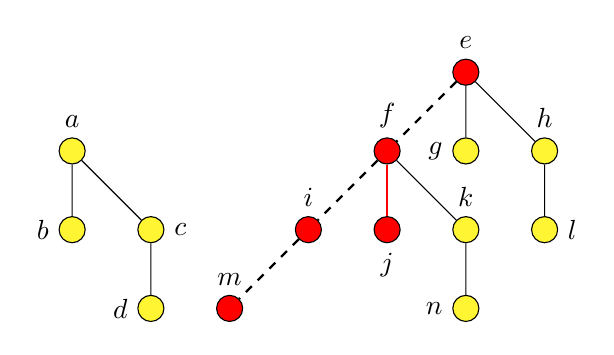
\begin{tikzpicture}
        \node[circle, draw, fill=yellow!80, label={90:$a$}] (a) at (0, 0) {};
        \node[circle, draw, fill=yellow!80, label={180:$b$}] (b) at (0, -1) {};
        \node[circle, draw, fill=yellow!80, label={0:$c$}] (c) at (1, -1) {};
        \node[circle, draw, fill=yellow!80, label={180:$d$}] (d) at (1, -2) {};
        
        \draw (a) to (b)
            (a) to (c)
            (c) to (d);
            
        \node[circle, draw, fill=red, label={90:$e$}] (e) at (5, 1) {};
        \node[circle, draw, fill=red, label={90:$f$}] (f) at (4, 0) {};
        \node[circle, draw, fill=yellow!80, label={180:$g$}] (g) at (5, 0) {};
        \node[circle, draw, fill=yellow!80, label={90:$h$}] (h) at (6, 0) {};
        \node[circle, draw, fill=red, label={90:$i$}] (i) at (3, -1) {};
        \node[circle, draw, fill=red, label={-90:$j$}] (j) at (4, -1) {};
        \node[circle, draw, fill=yellow!80, label={90:$k$}] (k) at (5, -1) {};
        \node[circle, draw, fill=yellow!80, label={0:$l$}] (l) at (6, -1) {};
        \node[circle, draw, fill=red, label={90:$m$}] (m) at (2, -2) {};
        \node[circle, draw, fill=yellow!80, label={180:$n$}] (n) at (5, -2) {};

        \draw[thick, dashed] (e) to (f)
            (f) to (i)
            (i) to (m);
        \draw[red, thick] (f) to (j);
        \draw (e) to (g)
            (e) to (h)
            (f) to (k)
            (h) to (l)
            (k) to (n);
    \end{tikzpicture}
\end{figure}
\noindent Now, we have visited $j$. We continue on, finding new vertices and backtracking until we have completely visited all the vertices in this connected component.
\begin{figure}[H]
    \centering
    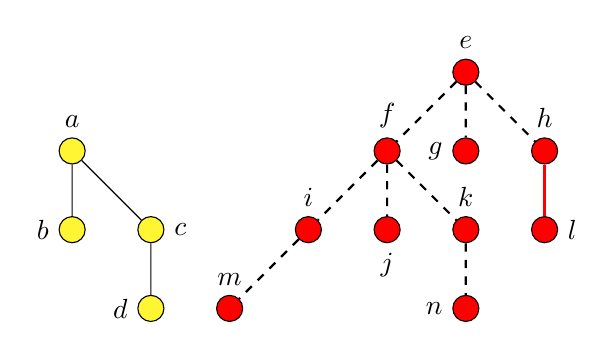
\begin{tikzpicture}
        \node[circle, draw, fill=yellow!80, label={90:$a$}] (a) at (0, 0) {};
        \node[circle, draw, fill=yellow!80, label={180:$b$}] (b) at (0, -1) {};
        \node[circle, draw, fill=yellow!80, label={0:$c$}] (c) at (1, -1) {};
        \node[circle, draw, fill=yellow!80, label={180:$d$}] (d) at (1, -2) {};
        
        \draw (a) to (b)
            (a) to (c)
            (c) to (d);
        
        \node[circle, draw, fill=red, label={90:$e$}] (e) at (5, 1) {};
        \node[circle, draw, fill=red, label={90:$f$}] (f) at (4, 0) {};
        \node[circle, draw, fill=red, label={180:$g$}] (g) at (5, 0) {};
        \node[circle, draw, fill=red, label={90:$h$}] (h) at (6, 0) {};
        \node[circle, draw, fill=red, label={90:$i$}] (i) at (3, -1) {};
        \node[circle, draw, fill=red, label={-90:$j$}] (j) at (4, -1) {};
        \node[circle, draw, fill=red, label={90:$k$}] (k) at (5, -1) {};
        \node[circle, draw, fill=red, label={0:$l$}] (l) at (6, -1) {};
        \node[circle, draw, fill=red, label={90:$m$}] (m) at (2, -2) {};
        \node[circle, draw, fill=red, label={180:$n$}] (n) at (5, -2) {};
        
        \draw[thick, dashed] (e) to (f)
            (f) to (i)
            (i) to (m)
            (f) to (j)
            (e) to (g)
            (e) to (h)
            (f) to (k)
            (k) to (n);
        \draw[red, thick] (h) to (l);
    \end{tikzpicture}
\end{figure}
\noindent Since we have visited all the edges in the right connected component, we randomly choose a vertex that has not yet been visited. Here, we choose $a$.
\begin{figure}[H]
    \centering
    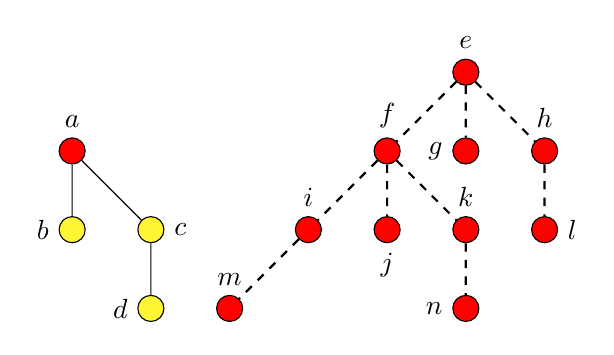
\begin{tikzpicture}
        \node[circle, draw, fill=red, label={90:$a$}] (a) at (0, 0) {};
        \node[circle, draw, fill=yellow!80, label={180:$b$}] (b) at (0, -1) {};
        \node[circle, draw, fill=yellow!80, label={0:$c$}] (c) at (1, -1) {};
        \node[circle, draw, fill=yellow!80, label={180:$d$}] (d) at (1, -2) {};
        
        \draw (a) to (b)
            (a) to (c)
            (c) to (d);
        
        \node[circle, draw, fill=red, label={90:$e$}] (e) at (5, 1) {};
        \node[circle, draw, fill=red, label={90:$f$}] (f) at (4, 0) {};
        \node[circle, draw, fill=red, label={180:$g$}] (g) at (5, 0) {};
        \node[circle, draw, fill=red, label={90:$h$}] (h) at (6, 0) {};
        \node[circle, draw, fill=red, label={90:$i$}] (i) at (3, -1) {};
        \node[circle, draw, fill=red, label={-90:$j$}] (j) at (4, -1) {};
        \node[circle, draw, fill=red, label={90:$k$}] (k) at (5, -1) {};
        \node[circle, draw, fill=red, label={0:$l$}] (l) at (6, -1) {};
        \node[circle, draw, fill=red, label={90:$m$}] (m) at (2, -2) {};
        \node[circle, draw, fill=red, label={180:$n$}] (n) at (5, -2) {};
        
        \draw[thick, dashed] (e) to (f)
            (f) to (i)
            (i) to (m)
            (f) to (j)
            (e) to (g)
            (e) to (h)
            (f) to (k)
            (k) to (n)
            (h) to (l);
    \end{tikzpicture}
\end{figure}
\noindent We find all the vertices we can visit from this vertex like we did before.
\begin{figure}[H]
    \centering
    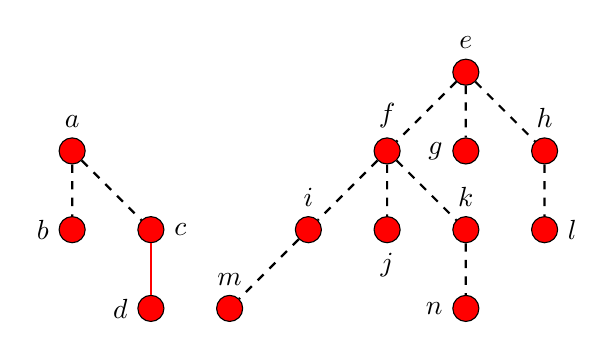
\begin{tikzpicture}
        \node[circle, draw, fill=red, label={90:$a$}] (a) at (0, 0) {};
        \node[circle, draw, fill=red, label={180:$b$}] (b) at (0, -1) {};
        \node[circle, draw, fill=red, label={0:$c$}] (c) at (1, -1) {};
        \node[circle, draw, fill=red, label={180:$d$}] (d) at (1, -2) {};
        
        \draw[thick, dashed] (a) to (b)
            (a) to (c);
        \draw[thick, red] (c) to (d);
        
        \node[circle, draw, fill=red, label={90:$e$}] (e) at (5, 1) {};
        \node[circle, draw, fill=red, label={90:$f$}] (f) at (4, 0) {};
        \node[circle, draw, fill=red, label={180:$g$}] (g) at (5, 0) {};
        \node[circle, draw, fill=red, label={90:$h$}] (h) at (6, 0) {};
        \node[circle, draw, fill=red, label={90:$i$}] (i) at (3, -1) {};
        \node[circle, draw, fill=red, label={-90:$j$}] (j) at (4, -1) {};
        \node[circle, draw, fill=red, label={90:$k$}] (k) at (5, -1) {};
        \node[circle, draw, fill=red, label={0:$l$}] (l) at (6, -1) {};
        \node[circle, draw, fill=red, label={90:$m$}] (m) at (2, -2) {};
        \node[circle, draw, fill=red, label={180:$n$}] (n) at (5, -2) {};
        
        \draw[thick, dashed] (e) to (f)
            (f) to (i)
            (i) to (m)
            (f) to (j)
            (e) to (g)
            (e) to (h)
            (f) to (k)
            (k) to (n)
            (h) to (l);
    \end{tikzpicture}
\end{figure}
\noindent We have now visited all the vertices, so the depth first search is complete.

The edges we traverse during depth-first search form a \emph{spanning tree} (or a forest if the graph is not connected). A spanning tree of a graph is a tree composed of all the vertices and some (or perhaps all) of the edges of the graph. Spanning trees that are found through a depth-first search traversal are called \emph{depth-first spanning trees}.

We will show how to form a spanning tree in the example below. We start the traversal at vertex $b$.
\begin{figure}[H]
    \centering
    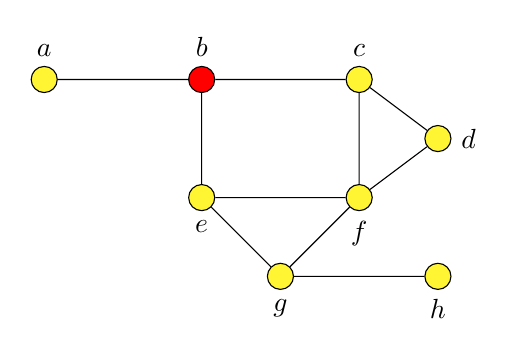
\begin{tikzpicture}
        \node[circle, draw, fill=yellow!80, label={90:$a$}] (a) at (0, -.5) {};
        \node[circle, draw, fill=red, label={90:$b$}] (b) at (2, -.5) {};
        \node[circle, draw, fill=yellow!80, label={90:$c$}] (c) at (4, -.5) {};
        \node[circle, draw, fill=yellow!80, label={0:$d$}] (d) at (5, -1.25) {};
        \node[circle, draw, fill=yellow!80, label={-90:$e$}] (e) at (2, -2) {};
        \node[circle, draw, fill=yellow!80, label={-90:$f$}] (f) at (4, -2) {};
        \node[circle, draw, fill=yellow!80, label={-90:$g$}] (g) at (3, -3) {};
        \node[circle, draw, fill=yellow!80, label={-90:$h$}] (h) at (5, -3) {};

        \draw (a) to (b)
            (b) to (c)
            (c) to (d)
            (c) to (f)
            (d) to (f)
            (b) to (e)
            (e) to (f)
            (e) to (g)
            (f) to (g)
            (g) to (h);
    \end{tikzpicture}
    \caption{An undirected graph being visited by depth-first search.}
\end{figure}
\noindent The vertex in red is the current vertex for the depth-first search (in order to find the minimum spanning tree). Like before, we will take some edge to find unvisited vertices. In this case, we take the edge to $c$.
\begin{figure}[H]
    \centering
    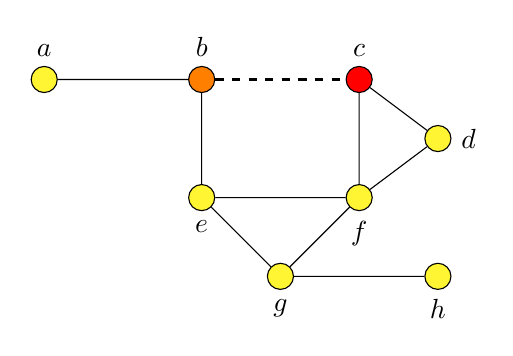
\begin{tikzpicture}
        \node[circle, draw, fill=yellow!80, label={90:$a$}] (a) at (0, -.5) {};
        \node[circle, draw, fill=orange, label={90:$b$}] (b) at (2, -.5) {};
        \node[circle, draw, fill=red, label={90:$c$}] (c) at (4, -.5) {};
        \node[circle, draw, fill=yellow!80, label={0:$d$}] (d) at (5, -1.25) {};
        \node[circle, draw, fill=yellow!80, label={-90:$e$}] (e) at (2, -2) {};
        \node[circle, draw, fill=yellow!80, label={-90:$f$}] (f) at (4, -2) {};
        \node[circle, draw, fill=yellow!80, label={-90:$g$}] (g) at (3, -3) {};
        \node[circle, draw, fill=yellow!80, label={-90:$h$}] (h) at (5, -3) {};

        \draw[dashed, thick] (b) to (c);
        \draw (a) to (b)
            (c) to (d)
            (c) to (f)
            (d) to (f)
            (b) to (e)
            (e) to (f)
            (e) to (g)
            (f) to (g)
            (g) to (h);
    \end{tikzpicture}
\end{figure}
\noindent The vertices in orange are previously visited vertices. Dashed edges have been taken. We continue the depth-first search algorithm and find another unvisited vertex from the current vertex, this time visiting $f$.
\begin{figure}[H]
    \centering
    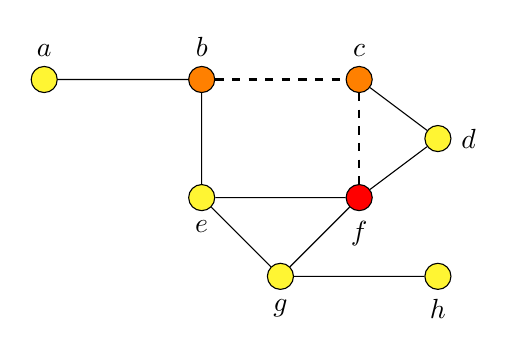
\begin{tikzpicture}
        \node[circle, draw, fill=yellow!80, label={90:$a$}] (a) at (0, -.5) {};
        \node[circle, draw, fill=orange, label={90:$b$}] (b) at (2, -.5) {};
        \node[circle, draw, fill=orange, label={90:$c$}] (c) at (4, -.5) {};
        \node[circle, draw, fill=yellow!80, label={0:$d$}] (d) at (5, -1.25) {};
        \node[circle, draw, fill=yellow!80, label={-90:$e$}] (e) at (2, -2) {};
        \node[circle, draw, fill=red, label={-90:$f$}] (f) at (4, -2) {};
        \node[circle, draw, fill=yellow!80, label={-90:$g$}] (g) at (3, -3) {};
        \node[circle, draw, fill=yellow!80, label={-90:$h$}] (h) at (5, -3) {};

        \draw[thick, dashed] (b) to (c)
            (c) to (f);
        \draw (a) to (b)
            (c) to (d)
            (b) to (e)
            (d) to (f)
            (e) to (f)
            (e) to (g)
            (f) to (g)
            (g) to (h);
    \end{tikzpicture}
\end{figure}
\noindent From the current vertex $f$, we find the unvisited vertex $d$.
\begin{figure}[H]
    \centering
    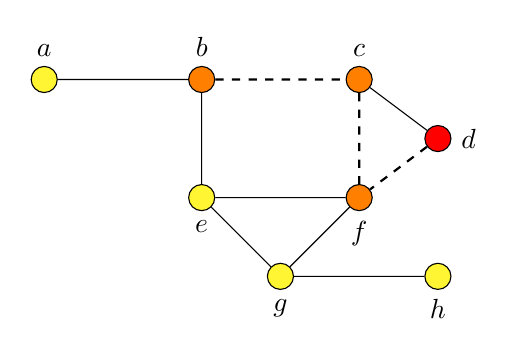
\begin{tikzpicture}
        \node[circle, draw, fill=yellow!80, label={90:$a$}] (a) at (0, -.5) {};
        \node[circle, draw, fill=orange, label={90:$b$}] (b) at (2, -.5) {};
        \node[circle, draw, fill=orange, label={90:$c$}] (c) at (4, -.5) {};
        \node[circle, draw, fill=red, label={0:$d$}] (d) at (5, -1.25) {};
        \node[circle, draw, fill=yellow!80, label={-90:$e$}] (e) at (2, -2) {};
        \node[circle, draw, fill=orange, label={-90:$f$}] (f) at (4, -2) {};
        \node[circle, draw, fill=yellow!80, label={-90:$g$}] (g) at (3, -3) {};
        \node[circle, draw, fill=yellow!80, label={-90:$h$}] (h) at (5, -3) {};

        \draw[thick, dashed] (b) to (c)
            (c) to (f)
            (d) to (f);
        \draw (a) to (b)
            (c) to (d)
            (b) to (e)
            (e) to (f)
            (e) to (g)
            (f) to (g)
            (g) to (h);
    \end{tikzpicture}
\end{figure}
\noindent There is only one edge that we haven't taken that $d$ is incident to- it goes from $d$ to $c$. However, $c$ has already been visited, so we have exhausted this vertex. We then backtrack and consider the previous vertex $f$.
\begin{figure}[H]
    \centering
    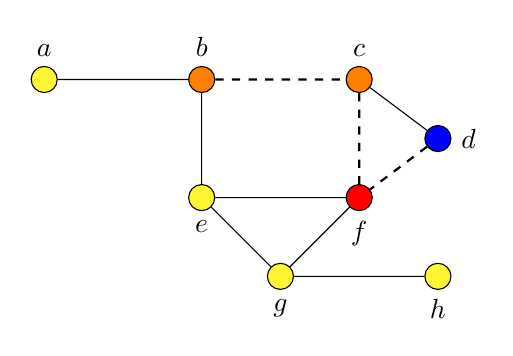
\begin{tikzpicture}
        \node[circle, draw, fill=yellow!80, label={90:$a$}] (a) at (0, -.5) {};
        \node[circle, draw, fill=orange, label={90:$b$}] (b) at (2, -.5) {};
        \node[circle, draw, fill=orange, label={90:$c$}] (c) at (4, -.5) {};
        \node[circle, draw, fill=blue, label={0:$d$}] (d) at (5, -1.25) {};
        \node[circle, draw, fill=yellow!80, label={-90:$e$}] (e) at (2, -2) {};
        \node[circle, draw, fill=red, label={-90:$f$}] (f) at (4, -2) {};
        \node[circle, draw, fill=yellow!80, label={-90:$g$}] (g) at (3, -3) {};
        \node[circle, draw, fill=yellow!80, label={-90:$h$}] (h) at (5, -3) {};

        \draw[thick, dashed] (b) to (c)
            (d) to (f)
            (c) to (f);
        \draw (a) to (b)
            (c) to (d)
            (b) to (e)
            (e) to (f)
            (e) to (g)
            (f) to (g)
            (g) to (h);
    \end{tikzpicture}
\end{figure}
\noindent The vertices in blue are vertices such that all of their edges have been completely explored- these vertices have been exhausted and we do not need to consider any edges from this vertex from this point. From $f$, there is an edge that takes us to  $g$, an unvisited vertex. So, we take this edge and visit $g$.
\begin{figure}[H]
    \centering
    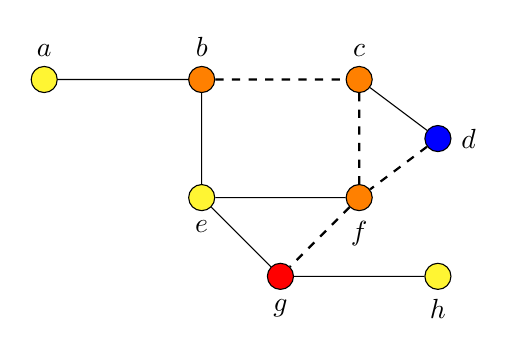
\begin{tikzpicture}
        \node[circle, draw, fill=yellow!80, label={90:$a$}] (a) at (0, -.5) {};
        \node[circle, draw, fill=orange, label={90:$b$}] (b) at (2, -.5) {};
        \node[circle, draw, fill=orange, label={90:$c$}] (c) at (4, -.5) {};
        \node[circle, draw, fill=blue, label={0:$d$}] (d) at (5, -1.25) {};
        \node[circle, draw, fill=yellow!80, label={-90:$e$}] (e) at (2, -2) {};
        \node[circle, draw, fill=orange, label={-90:$f$}] (f) at (4, -2) {};
        \node[circle, draw, fill=red, label={-90:$g$}] (g) at (3, -3) {};
        \node[circle, draw, fill=yellow!80, label={-90:$h$}] (h) at (5, -3) {};

        \draw[thick, dashed] (b) to (c)
            (d) to (f)
            (c) to (f)
            (f) to (g);
        \draw (a) to (b)
            (c) to (d)
            (b) to (e)
            (e) to (f)
            (e) to (g)
            (g) to (h);
    \end{tikzpicture}
\end{figure}
\noindent From vertex $g$, we find the unvisited vertex $h$.
\begin{figure}[H]
    \centering
    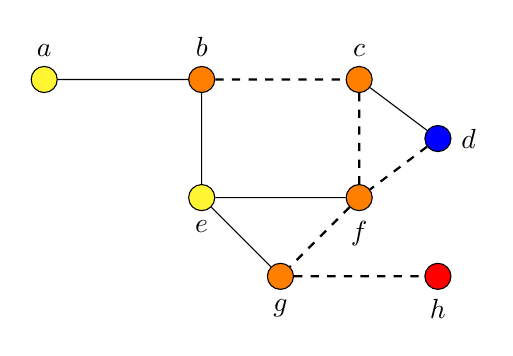
\begin{tikzpicture}
        \node[circle, draw, fill=yellow!80, label={90:$a$}] (a) at (0, -.5) {};
        \node[circle, draw, fill=orange, label={90:$b$}] (b) at (2, -.5) {};
        \node[circle, draw, fill=orange, label={90:$c$}] (c) at (4, -.5) {};
        \node[circle, draw, fill=blue, label={0:$d$}] (d) at (5, -1.25) {};
        \node[circle, draw, fill=yellow!80, label={-90:$e$}] (e) at (2, -2) {};
        \node[circle, draw, fill=orange, label={-90:$f$}] (f) at (4, -2) {};
        \node[circle, draw, fill=orange, label={-90:$g$}] (g) at (3, -3) {};
        \node[circle, draw, fill=red, label={-90:$h$}] (h) at (5, -3) {};

        \draw[thick, dashed] (b) to (c)
            (d) to (f)
            (c) to (f)
            (f) to (g)
            (g) to (h);
        \draw (a) to (b)
            (c) to (d)
            (b) to (e)
            (e) to (f)
            (e) to (g);
    \end{tikzpicture}
\end{figure}
\noindent There is no edge from $h$ that we haven't taken. So, we mark this vertex as exhausted and backtrack.
\begin{figure}[H]
    \centering
    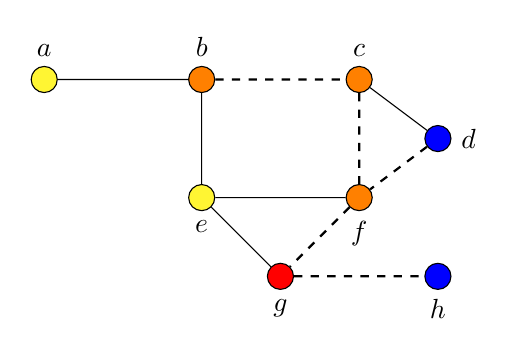
\begin{tikzpicture}
        \node[circle, draw, fill=yellow!80, label={90:$a$}] (a) at (0, -.5) {};
        \node[circle, draw, fill=orange, label={90:$b$}] (b) at (2, -.5) {};
        \node[circle, draw, fill=orange, label={90:$c$}] (c) at (4, -.5) {};
        \node[circle, draw, fill=blue, label={0:$d$}] (d) at (5, -1.25) {};
        \node[circle, draw, fill=yellow!80, label={-90:$e$}] (e) at (2, -2) {};
        \node[circle, draw, fill=orange, label={-90:$f$}] (f) at (4, -2) {};
        \node[circle, draw, fill=red, label={-90:$g$}] (g) at (3, -3) {};
        \node[circle, draw, fill=blue, label={-90:$h$}] (h) at (5, -3) {};

        \draw[thick, dashed] (b) to (c)
            (d) to (f)
            (c) to (f)
            (g) to (h)
            (f) to (g);
        \draw (a) to (b)
            (c) to (d)
            (b) to (e)
            (e) to (f)
            (e) to (g);
    \end{tikzpicture}
\end{figure}
\noindent From the vertex $g$, we can find an edge to the unvisited vertex $e$, so we take it.
\begin{figure}[H]
    \centering
    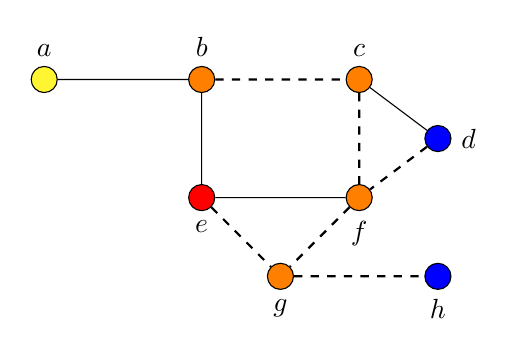
\begin{tikzpicture}
        \node[circle, draw, fill=yellow!80, label={90:$a$}] (a) at (0, -.5) {};
        \node[circle, draw, fill=orange, label={90:$b$}] (b) at (2, -.5) {};
        \node[circle, draw, fill=orange, label={90:$c$}] (c) at (4, -.5) {};
        \node[circle, draw, fill=blue, label={0:$d$}] (d) at (5, -1.25) {};
        \node[circle, draw, fill=red, label={-90:$e$}] (e) at (2, -2) {};
        \node[circle, draw, fill=orange, label={-90:$f$}] (f) at (4, -2) {};
        \node[circle, draw, fill=orange, label={-90:$g$}] (g) at (3, -3) {};
        \node[circle, draw, fill=blue, label={-90:$h$}] (h) at (5, -3) {};

        \draw[thick, dashed] (b) to (c)
            (d) to (f)
            (c) to (f)
            (g) to (h)
            (f) to (g)
            (e) to (g);
        \draw (a) to (b)
            (c) to (d)
            (b) to (e)
            (e) to (f);
    \end{tikzpicture}
\end{figure}
\noindent There are two edges from $e$ that we haven't taken- one to $f$ and another to $b$. However, both of these vertices have already been visited. So, we mark $e$ as exhausted and backtrack to $g$.
\begin{figure}[H]
    \centering
    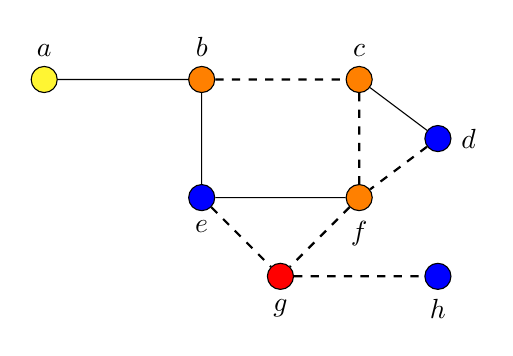
\begin{tikzpicture}
        \node[circle, draw, fill=yellow!80, label={90:$a$}] (a) at (0, -.5) {};
        \node[circle, draw, fill=orange, label={90:$b$}] (b) at (2, -.5) {};
        \node[circle, draw, fill=orange, label={90:$c$}] (c) at (4, -.5) {};
        \node[circle, draw, fill=blue, label={0:$d$}] (d) at (5, -1.25) {};
        \node[circle, draw, fill=blue, label={-90:$e$}] (e) at (2, -2) {};
        \node[circle, draw, fill=orange, label={-90:$f$}] (f) at (4, -2) {};
        \node[circle, draw, fill=red, label={-90:$g$}] (g) at (3, -3) {};
        \node[circle, draw, fill=blue, label={-90:$h$}] (h) at (5, -3) {};

        \draw[thick, dashed] (b) to (c)
            (d) to (f)
            (c) to (f)
            (g) to (h)
            (f) to (g)
            (e) to (g);
        \draw (a) to (b)
            (c) to (d)
            (b) to (e)
            (e) to (f);
    \end{tikzpicture}
\end{figure}
\noindent There is no edge left to visit from $g$, so we mark it as exhausted and backtrack.
\begin{figure}[H]
    \centering
    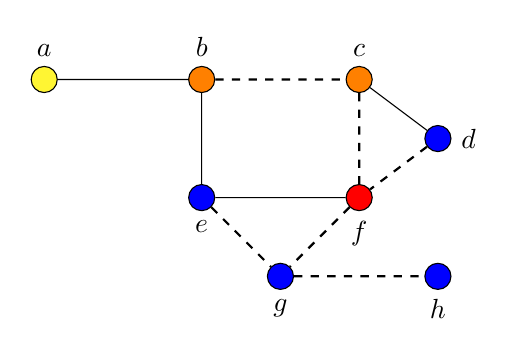
\begin{tikzpicture}
        \node[circle, draw, fill=yellow!80, label={90:$a$}] (a) at (0, -.5) {};
        \node[circle, draw, fill=orange, label={90:$b$}] (b) at (2, -.5) {};
        \node[circle, draw, fill=orange, label={90:$c$}] (c) at (4, -.5) {};
        \node[circle, draw, fill=blue, label={0:$d$}] (d) at (5, -1.25) {};
        \node[circle, draw, fill=blue, label={-90:$e$}] (e) at (2, -2) {};
        \node[circle, draw, fill=red, label={-90:$f$}] (f) at (4, -2) {};
        \node[circle, draw, fill=blue, label={-90:$g$}] (g) at (3, -3) {};
        \node[circle, draw, fill=blue, label={-90:$h$}] (h) at (5, -3) {};
        
        \draw[thick, dashed] (b) to (c)
            (d) to (f)
            (c) to (f)
            (g) to (h)
            (f) to (g)
            (e) to (g);
        \draw (a) to (b)
            (c) to (d)
            (b) to (e)
            (e) to (f);
    \end{tikzpicture}
\end{figure}
\noindent From $f$, there is only one edge that we haven't considered- it goes to $e$. But, we have already visited $e$. So, we mark this vertex as exhausted and backtrack again, to $c$.
\begin{figure}[H]
    \centering
    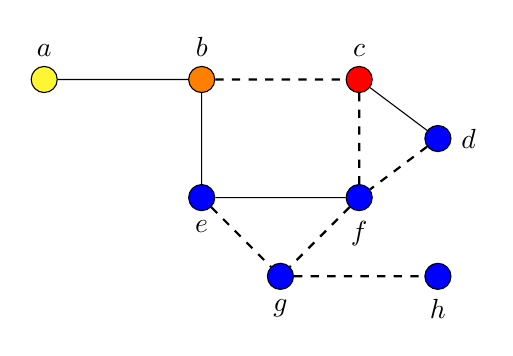
\begin{tikzpicture}
        \node[circle, draw, fill=yellow!80, label={90:$a$}] (a) at (0, -.5) {};
        \node[circle, draw, fill=orange, label={90:$b$}] (b) at (2, -.5) {};
        \node[circle, draw, fill=red, label={90:$c$}] (c) at (4, -.5) {};
        \node[circle, draw, fill=blue, label={0:$d$}] (d) at (5, -1.25) {};
        \node[circle, draw, fill=blue, label={-90:$e$}] (e) at (2, -2) {};
        \node[circle, draw, fill=blue, label={-90:$f$}] (f) at (4, -2) {};
        \node[circle, draw, fill=blue, label={-90:$g$}] (g) at (3, -3) {};
        \node[circle, draw, fill=blue, label={-90:$h$}] (h) at (5, -3) {};

        \draw[thick, dashed] (b) to (c)
            (d) to (f)
            (c) to (f)
            (g) to (h)
            (f) to (g)
            (e) to (g);
        \draw (a) to (b)
            (c) to (d)
            (b) to (e)
            (e) to (f);
    \end{tikzpicture}
\end{figure}
\noindent Like before, there is no edge we can take from $c$ to find an unvisited vertex. So, we mark this vertex as exhausted and backtrack again, to $b$.
\begin{figure}[H]
    \centering
    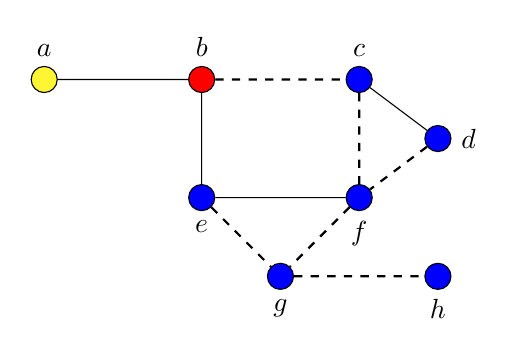
\begin{tikzpicture}
        \node[circle, draw, fill=yellow!80, label={90:$a$}] (a) at (0, -.5) {};
        \node[circle, draw, fill=red, label={90:$b$}] (b) at (2, -.5) {};
        \node[circle, draw, fill=blue, label={90:$c$}] (c) at (4, -.5) {};
        \node[circle, draw, fill=blue, label={0:$d$}] (d) at (5, -1.25) {};
        \node[circle, draw, fill=blue, label={-90:$e$}] (e) at (2, -2) {};
        \node[circle, draw, fill=blue, label={-90:$f$}] (f) at (4, -2) {};
        \node[circle, draw, fill=blue, label={-90:$g$}] (g) at (3, -3) {};
        \node[circle, draw, fill=blue, label={-90:$h$}] (h) at (5, -3) {};

        \draw[thick, dashed] (b) to (c)
            (d) to (f)
            (c) to (f)
            (g) to (h)
            (f) to (g)
            (e) to (g);
        \draw (a) to (b)
            (c) to (d)
            (b) to (e)
            (e) to (f);
    \end{tikzpicture}
\end{figure}
\noindent Finally, we can find an edge from the current vertex that goes to an unvisited vertex- it goes from $b$ to $a$.
\begin{figure}[H]
    \centering
    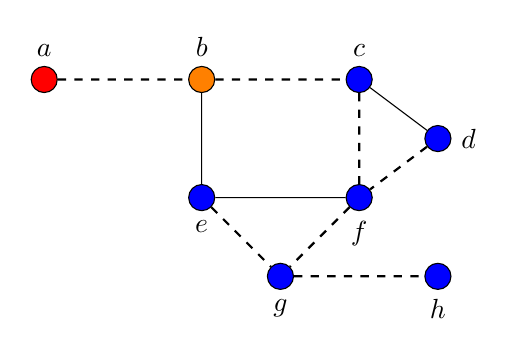
\begin{tikzpicture}
        \node[circle, draw, fill=red, label={90:$a$}] (a) at (0, -.5) {};
        \node[circle, draw, fill=orange, label={90:$b$}] (b) at (2, -.5) {};
        \node[circle, draw, fill=blue, label={90:$c$}] (c) at (4, -.5) {};
        \node[circle, draw, fill=blue, label={0:$d$}] (d) at (5, -1.25) {};
        \node[circle, draw, fill=blue, label={-90:$e$}] (e) at (2, -2) {};
        \node[circle, draw, fill=blue, label={-90:$f$}] (f) at (4, -2) {};
        \node[circle, draw, fill=blue, label={-90:$g$}] (g) at (3, -3) {};
        \node[circle, draw, fill=blue, label={-90:$h$}] (h) at (5, -3) {};

        \draw[thick, dashed] (b) to (c)
            (d) to (f)
            (c) to (f)
            (g) to (h)
            (f) to (g)
            (e) to (g)
            (a) to (b);
        \draw (c) to (d)
            (b) to (e)
            (e) to (f);
    \end{tikzpicture}
\end{figure}
\noindent From $a$, there is no further edge we can take. So, we mark this vertex as exhausted and backtrack to $b$.
\begin{figure}[H]
    \centering
    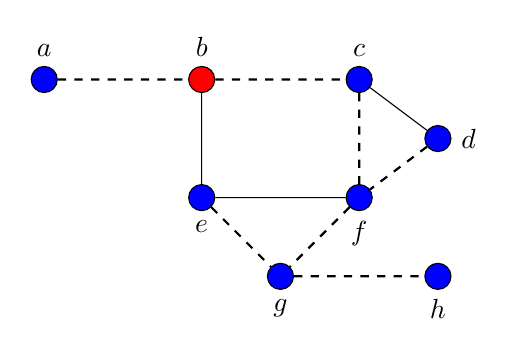
\begin{tikzpicture}
        \node[circle, draw, fill=blue, label={90:$a$}] (a) at (0, -.5) {};
        \node[circle, draw, fill=red, label={90:$b$}] (b) at (2, -.5) {};
        \node[circle, draw, fill=blue, label={90:$c$}] (c) at (4, -.5) {};
        \node[circle, draw, fill=blue, label={0:$d$}] (d) at (5, -1.25) {};
        \node[circle, draw, fill=blue, label={-90:$e$}] (e) at (2, -2) {};
        \node[circle, draw, fill=blue, label={-90:$f$}] (f) at (4, -2) {};
        \node[circle, draw, fill=blue, label={-90:$g$}] (g) at (3, -3) {};
        \node[circle, draw, fill=blue, label={-90:$h$}] (h) at (5, -3) {};

        \draw[thick, dashed] (b) to (c)
            (d) to (f)
            (c) to (f)
            (g) to (h)
            (f) to (g)
            (e) to (g)
            (a) to (b);
        \draw (c) to (d)
            (b) to (e)
            (e) to (f);
    \end{tikzpicture}
\end{figure}
\noindent From $b$, there is no edge we can take to find an unvisited vertex, so we mark $b$ as exhausted.
\begin{figure}[H]
    \centering
    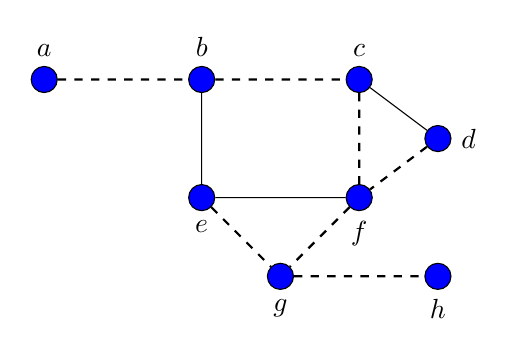
\begin{tikzpicture}
        \node[circle, draw, fill=blue, label={90:$a$}] (a) at (0, -.5) {};
        \node[circle, draw, fill=blue, label={90:$b$}] (b) at (2, -.5) {};
        \node[circle, draw, fill=blue, label={90:$c$}] (c) at (4, -.5) {};
        \node[circle, draw, fill=blue, label={0:$d$}] (d) at (5, -1.25) {};
        \node[circle, draw, fill=blue, label={-90:$e$}] (e) at (2, -2) {};
        \node[circle, draw, fill=blue, label={-90:$f$}] (f) at (4, -2) {};
        \node[circle, draw, fill=blue, label={-90:$g$}] (g) at (3, -3) {};
        \node[circle, draw, fill=blue, label={-90:$h$}] (h) at (5, -3) {};
        
        \draw[thick, dashed] (b) to (c)
            (d) to (f)
            (c) to (f)
            (g) to (h)
            (f) to (g)
            (e) to (g)
            (a) to (b);
        \draw (c) to (d)
            (b) to (e)
            (e) to (f);
    \end{tikzpicture}
\end{figure}
\noindent We cannot backtrack since $b$ was the first edge, so we have found a spanning tree.
\begin{figure}[H]
    \centering
    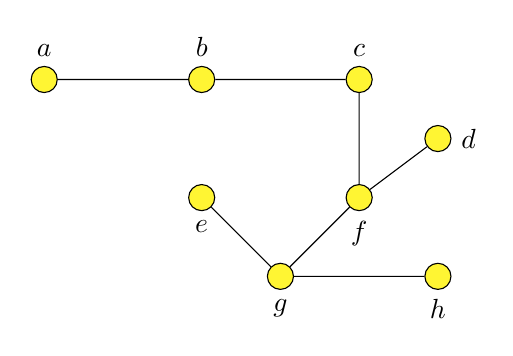
\begin{tikzpicture}
        \node[circle, draw, fill=yellow!80, label={90:$a$}] (a) at (0, -.5) {};
        \node[circle, draw, fill=yellow!80, label={90:$b$}] (b) at (2, -.5) {};
        \node[circle, draw, fill=yellow!80, label={90:$c$}] (c) at (4, -.5) {};
        \node[circle, draw, fill=yellow!80, label={0:$d$}] (d) at (5, -1.25) {};
        \node[circle, draw, fill=yellow!80, label={-90:$e$}] (e) at (2, -2) {};
        \node[circle, draw, fill=yellow!80, label={-90:$f$}] (f) at (4, -2) {};
        \node[circle, draw, fill=yellow!80, label={-90:$g$}] (g) at (3, -3) {};
        \node[circle, draw, fill=yellow!80, label={-90:$h$}] (h) at (5, -3) {};

        \draw (b) to (c)
            (d) to (f)
            (c) to (f)
            (g) to (h)
            (f) to (g)
            (e) to (g)
            (a) to (b);
    \end{tikzpicture}
    \caption{A spanning tree of the graph above, found using depth-first search.}
\end{figure}
\noindent We made many choices when selecting the edges from a vertex to another. So, there is no unique depth-first spanning tree.

The following is the implementation of depth first search.
\lstinputlisting[language=pseudocode]{src/depthFirstSearch.psc}

We now analyse the complexity of depth first search using adjacency lists. We visit each vertex once, and each element in the adjacency list is processed once. That is, each edge is visited once (or twice in the case of an undirected graph). So, the overall complexity is $O(|V| + |E|)$. We can adapt it using the adjacency matrix representation, but then it is $O(|V|^2)$ since we need to look at every entry of the adjacency matrix.

There are many applications of depth-first search. It can be used to determine if a graph is connected; to identify the connected components of a graph; to determine if a graph contains a cycle; and to determine if a graph is bipartile.

\subsection{Breadth First Search}
In depth-first search, we saw that we keep traversing in the same path until we cannot go any further. On the other hand, in breadth-first search, we visit all the edges of a particular vertex before visiting any vertices adjacent to them; the search fans out as widely as possible at each vertex. At every point, we keep a queue of vertices so we know the order in which we visit the vertices.

We show how this algorithm works by example. So, we start with an empty queue and a visited vertex $q$.
\begin{figure}[H]
    \centering
    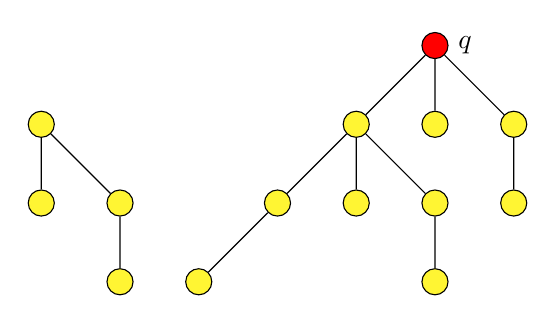
\begin{tikzpicture}
        \node[circle, draw, fill=yellow!80] (a) at (0, 0) {};
        \node[circle, draw, fill=yellow!80] (b) at (0, -1) {};
        \node[circle, draw, fill=yellow!80] (c) at (1, -1) {};
        \node[circle, draw, fill=yellow!80] (d) at (1, -2) {};
        
        \draw (a) to (b)
            (a) to (c)
            (c) to (d);
        
        \node[circle, draw, fill=red, label={0:$q$}] (e) at (5, 1) {};
        \node[circle, draw, fill=yellow!80] (f) at (4, 0) {};
        \node[circle, draw, fill=yellow!80] (g) at (5, 0) {};
        \node[circle, draw, fill=yellow!80] (h) at (6, 0) {};
        \node[circle, draw, fill=yellow!80] (i) at (3, -1) {};
        \node[circle, draw, fill=yellow!80] (j) at (4, -1) {};
        \node[circle, draw, fill=yellow!80] (k) at (5, -1) {};
        \node[circle, draw, fill=yellow!80] (l) at (6, -1) {};
        \node[circle, draw, fill=yellow!80] (m) at (2, -2) {};
        \node[circle, draw, fill=yellow!80] (n) at (5, -2) {};
        
        \draw (e) to (f)
            (e) to (g)
            (e) to (h)
            (f) to (i)
            (f) to (j)
            (f) to (k)
            (h) to (l)
            (i) to (m)
            (k) to (n);
    \end{tikzpicture}
    \caption{An undirected graph to be traversed via breadth-first search.}
\end{figure}
\noindent The visited vertices are in red, and the current edges are red. We find three edges here. So, we add the three vertices ($r$, $s$ and $t$) into the queue.
\begin{figure}[H]
    \centering
    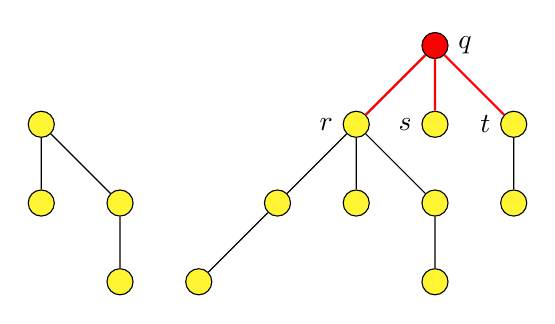
\begin{tikzpicture}
        \node[circle, draw, fill=yellow!80] (a) at (0, 0) {};
        \node[circle, draw, fill=yellow!80] (b) at (0, -1) {};
        \node[circle, draw, fill=yellow!80] (c) at (1, -1) {};
        \node[circle, draw, fill=yellow!80] (d) at (1, -2) {};
        
        \draw (a) to (b)
            (a) to (c)
            (c) to (d);
        
        \node[circle, draw, fill=red, label={0:$q$}] (e) at (5, 1) {};
        \node[circle, draw, fill=yellow!80, label={180:$r$}] (f) at (4, 0) {};
        \node[circle, draw, fill=yellow!80, label={180:$s$}] (g) at (5, 0) {};
        \node[circle, draw, fill=yellow!80, label={180:$t$}] (h) at (6, 0) {};
        \node[circle, draw, fill=yellow!80] (i) at (3, -1) {};
        \node[circle, draw, fill=yellow!80] (j) at (4, -1) {};
        \node[circle, draw, fill=yellow!80] (k) at (5, -1) {};
        \node[circle, draw, fill=yellow!80] (l) at (6, -1) {};
        \node[circle, draw, fill=yellow!80] (m) at (2, -2) {};
        \node[circle, draw, fill=yellow!80] (n) at (5, -2) {};
        
        \draw[red, thick] (e) to (f)
            (e) to (g)
            (e) to (h);
        \draw (f) to (i)
            (f) to (j)
            (f) to (k)
            (h) to (l)
            (i) to (m)
            (k) to (n);
    \end{tikzpicture}
    \caption{An undirected graph to be traversed via depth-first search.}
\end{figure}
\noindent The queue is now $\langle r, s, t \rangle$. We remove the first element from the queue and visit that vertex.
\begin{figure}[H]
    \centering
    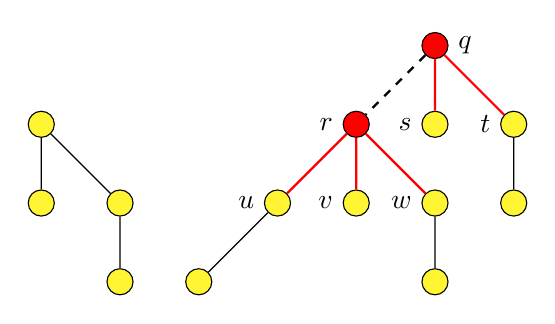
\begin{tikzpicture}
        \node[circle, draw, fill=yellow!80] (a) at (0, 0) {};
        \node[circle, draw, fill=yellow!80] (b) at (0, -1) {};
        \node[circle, draw, fill=yellow!80] (c) at (1, -1) {};
        \node[circle, draw, fill=yellow!80] (d) at (1, -2) {};
        
        \draw (a) to (b)
            (a) to (c)
            (c) to (d);
        
        \node[circle, draw, fill=red, label={0:$q$}] (e) at (5, 1) {};
        \node[circle, draw, fill=red, label={180:$r$}] (f) at (4, 0) {};
        \node[circle, draw, fill=yellow!80, label={180:$s$}] (g) at (5, 0) {};
        \node[circle, draw, fill=yellow!80, label={180:$t$}] (h) at (6, 0) {};
        \node[circle, draw, fill=yellow!80, label={180:$u$}] (i) at (3, -1) {};
        \node[circle, draw, fill=yellow!80, label={180:$v$}] (j) at (4, -1) {};
        \node[circle, draw, fill=yellow!80, label={180:$w$}] (k) at (5, -1) {};
        \node[circle, draw, fill=yellow!80] (l) at (6, -1) {};
        \node[circle, draw, fill=yellow!80] (m) at (2, -2) {};
        \node[circle, draw, fill=yellow!80] (n) at (5, -2) {};
        
        \draw[thick, dashed] (e) to (f);
        \draw[red, thick] (e) to (g)
            (e) to (h)
            (f) to (i)
            (f) to (j)
            (f) to (k);
        \draw (h) to (l)
            (i) to (m)
            (k) to (n);
    \end{tikzpicture}
\end{figure}
\noindent The visited edges are dashed. We now find 3 more vertices, so we add them to the queue as well. The queue is $\langle s, t, u, v, w \rangle$. We remove the first element from the queue and visit that vertex.
\begin{figure}[H]
    \centering
    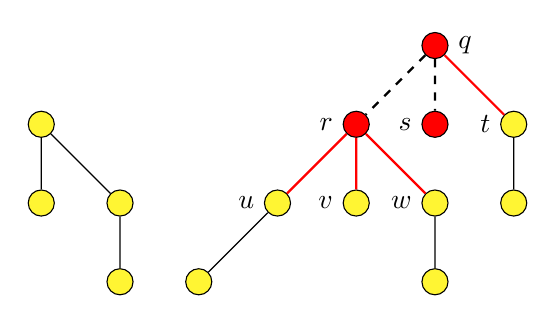
\begin{tikzpicture}
        \node[circle, draw, fill=yellow!80] (a) at (0, 0) {};
        \node[circle, draw, fill=yellow!80] (b) at (0, -1) {};
        \node[circle, draw, fill=yellow!80] (c) at (1, -1) {};
        \node[circle, draw, fill=yellow!80] (d) at (1, -2) {};
        
        \draw (a) to (b)
            (a) to (c)
            (c) to (d);
        
        \node[circle, draw, fill=red, label={0:$q$}] (e) at (5, 1) {};
        \node[circle, draw, fill=red, label={180:$r$}] (f) at (4, 0) {};
        \node[circle, draw, fill=red, label={180:$s$}] (g) at (5, 0) {};
        \node[circle, draw, fill=yellow!80, label={180:$t$}] (h) at (6, 0) {};
        \node[circle, draw, fill=yellow!80, label={180:$u$}] (i) at (3, -1) {};
        \node[circle, draw, fill=yellow!80, label={180:$v$}] (j) at (4, -1) {};
        \node[circle, draw, fill=yellow!80, label={180:$w$}] (k) at (5, -1) {};
        \node[circle, draw, fill=yellow!80] (l) at (6, -1) {};
        \node[circle, draw, fill=yellow!80] (m) at (2, -2) {};
        \node[circle, draw, fill=yellow!80] (n) at (5, -2) {};
        
        \draw[thick, dashed] (e) to (f)
            (e) to (g);
        \draw[thick, red] (f) to (i)
            (f) to (j)
            (f) to (k)
            (e) to (h);
        \draw (h) to (l)
            (i) to (m)
            (k) to (n);
    \end{tikzpicture}
\end{figure}
\noindent There are no edges from $s$ that are to be visited, so the queue remains $\langle t, u, v, w \rangle$. We remove $t$ from the queue and visit that vertex.
\begin{figure}[H]
    \centering
    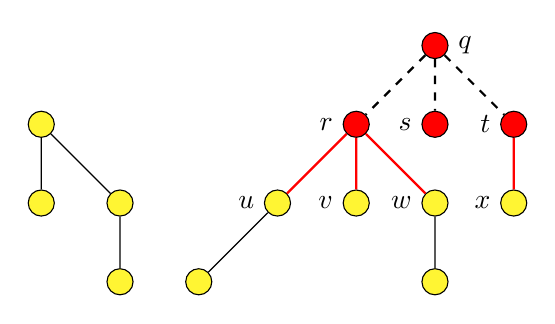
\begin{tikzpicture}
        \node[circle, draw, fill=yellow!80] (a) at (0, 0) {};
        \node[circle, draw, fill=yellow!80] (b) at (0, -1) {};
        \node[circle, draw, fill=yellow!80] (c) at (1, -1) {};
        \node[circle, draw, fill=yellow!80] (d) at (1, -2) {};
        
        \draw (a) to (b)
            (a) to (c)
            (c) to (d);
        
        \node[circle, draw, fill=red, label={0:$q$}] (e) at (5, 1) {};
        \node[circle, draw, fill=red, label={180:$r$}] (f) at (4, 0) {};
        \node[circle, draw, fill=red, label={180:$s$}] (g) at (5, 0) {};
        \node[circle, draw, fill=red, label={180:$t$}] (h) at (6, 0) {};
        \node[circle, draw, fill=yellow!80, label={180:$u$}] (i) at (3, -1) {};
        \node[circle, draw, fill=yellow!80, label={180:$v$}] (j) at (4, -1) {};
        \node[circle, draw, fill=yellow!80, label={180:$w$}] (k) at (5, -1) {};
        \node[circle, draw, fill=yellow!80, label={180:$x$}] (l) at (6, -1) {};
        \node[circle, draw, fill=yellow!80] (m) at (2, -2) {};
        \node[circle, draw, fill=yellow!80] (n) at (5, -2) {};
        
        \draw[thick, dashed] (e) to (f)
            (e) to (g)
            (e) to (h);
        \draw[red, thick] (f) to (i)
            (f) to (j)
            (f) to (k)
            (h) to (l);
        \draw (i) to (m)
            (k) to (n);
    \end{tikzpicture}
\end{figure}
\noindent We add $x$ to the queue now, so the queue is $\langle u, v, w, x \rangle$. We remove $u$ now and visit that vertex.
\begin{figure}[H]
    \centering
    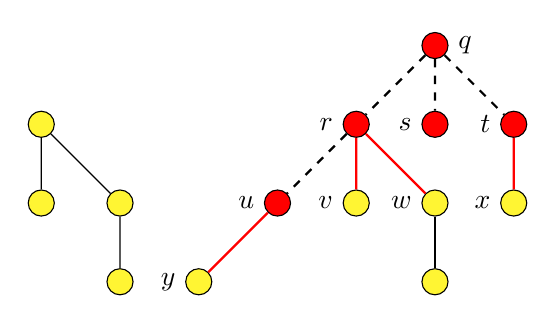
\begin{tikzpicture}
        \node[circle, draw, fill=yellow!80] (a) at (0, 0) {};
        \node[circle, draw, fill=yellow!80] (b) at (0, -1) {};
        \node[circle, draw, fill=yellow!80] (c) at (1, -1) {};
        \node[circle, draw, fill=yellow!80] (d) at (1, -2) {};
        
        \draw (a) to (b)
            (a) to (c)
            (c) to (d);
        
        \node[circle, draw, fill=red, label={0:$q$}] (e) at (5, 1) {};
        \node[circle, draw, fill=red, label={180:$r$}] (f) at (4, 0) {};
        \node[circle, draw, fill=red, label={180:$s$}] (g) at (5, 0) {};
        \node[circle, draw, fill=red, label={180:$t$}] (h) at (6, 0) {};
        \node[circle, draw, fill=red, label={180:$u$}] (i) at (3, -1) {};
        \node[circle, draw, fill=yellow!80, label={180:$v$}] (j) at (4, -1) {};
        \node[circle, draw, fill=yellow!80, label={180:$w$}] (k) at (5, -1) {};
        \node[circle, draw, fill=yellow!80, label={180:$x$}] (l) at (6, -1) {};
        \node[circle, draw, fill=yellow!80, label={180:$y$}] (m) at (2, -2) {};
        \node[circle, draw, fill=yellow!80] (n) at (5, -2) {};
        
        \draw[thick, dashed] (e) to (f)
            (e) to (g)
            (e) to (h)
            (f) to (i);
        \draw[red, thick] (f) to (j)
            (f) to (k)
            (h) to (l)
            (i) to (m);
        \draw (k) to (n);
    \end{tikzpicture}
\end{figure}
\noindent We add $y$ to the queue now. The queue is then $\langle v, w, x, y \rangle$. So, we remove $v$ and visit it.
\begin{figure}[H]
    \centering
    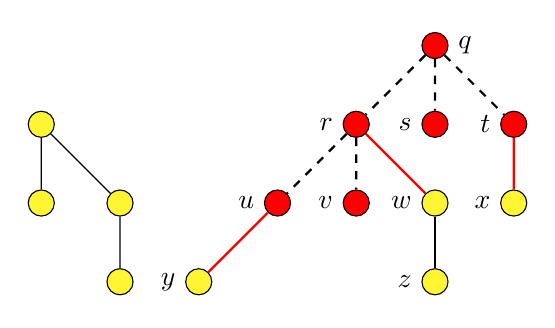
\begin{tikzpicture}
        \node[circle, draw, fill=yellow!80] (a) at (0, 0) {};
        \node[circle, draw, fill=yellow!80] (b) at (0, -1) {};
        \node[circle, draw, fill=yellow!80] (c) at (1, -1) {};
        \node[circle, draw, fill=yellow!80] (d) at (1, -2) {};
        
        \draw (a) to (b)
            (a) to (c)
            (c) to (d);
        
        \node[circle, draw, fill=red, label={0:$q$}] (e) at (5, 1) {};
        \node[circle, draw, fill=red, label={180:$r$}] (f) at (4, 0) {};
        \node[circle, draw, fill=red, label={180:$s$}] (g) at (5, 0) {};
        \node[circle, draw, fill=red, label={180:$t$}] (h) at (6, 0) {};
        \node[circle, draw, fill=red, label={180:$u$}] (i) at (3, -1) {};
        \node[circle, draw, fill=red, label={180:$v$}] (j) at (4, -1) {};
        \node[circle, draw, fill=yellow!80, label={180:$w$}] (k) at (5, -1) {};
        \node[circle, draw, fill=yellow!80, label={180:$x$}] (l) at (6, -1) {};
        \node[circle, draw, fill=yellow!80, label={180:$y$}] (m) at (2, -2) {};
        \node[circle, draw, fill=yellow!80, label={180:$z$}] (n) at (5, -2) {};
        
        \draw[thick, dashed] (e) to (f)
            (e) to (g)
            (e) to (h)
            (f) to (i)
            (f) to (j);
        \draw[red, thick] (f) to (k)
            (h) to (l)
            (i) to (m);
        \draw (k) to (n);
    \end{tikzpicture}
\end{figure}
\noindent There is no vertex to add here, so the queue remains $\langle w, x, y \rangle$. We can continue this process and find all the remaining vertices in the connected subgraph on the right.
\begin{figure}[H]
    \centering
    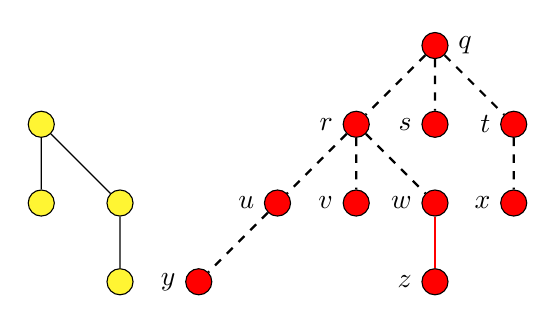
\begin{tikzpicture}
        \node[circle, draw, fill=yellow!80] (a) at (0, 0) {};
        \node[circle, draw, fill=yellow!80] (b) at (0, -1) {};
        \node[circle, draw, fill=yellow!80] (c) at (1, -1) {};
        \node[circle, draw, fill=yellow!80] (d) at (1, -2) {};
        
        \draw (a) to (b)
            (a) to (c)
            (c) to (d);
        
        \node[circle, draw, fill=red, label={0:$q$}] (e) at (5, 1) {};
        \node[circle, draw, fill=red, label={180:$r$}] (f) at (4, 0) {};
        \node[circle, draw, fill=red, label={180:$s$}] (g) at (5, 0) {};
        \node[circle, draw, fill=red, label={180:$t$}] (h) at (6, 0) {};
        \node[circle, draw, fill=red, label={180:$u$}] (i) at (3, -1) {};
        \node[circle, draw, fill=red, label={180:$v$}] (j) at (4, -1) {};
        \node[circle, draw, fill=red, label={180:$w$}] (k) at (5, -1) {};
        \node[circle, draw, fill=red, label={180:$x$}] (l) at (6, -1) {};
        \node[circle, draw, fill=red, label={180:$y$}] (m) at (2, -2) {};
        \node[circle, draw, fill=red, label={180:$z$}] (n) at (5, -2) {};
        
        \draw[thick, dashed] (e) to (f)
            (e) to (g)
            (e) to (h)
            (f) to (i)
            (f) to (j)
            (f) to (k)
            (h) to (l)
            (i) to (m);
        \draw[thick, red] (k) to (n);
    \end{tikzpicture}
\end{figure}
\noindent There are still unvisited vertices, so we select an unvisited vertex.
\begin{figure}[H]
    \centering
    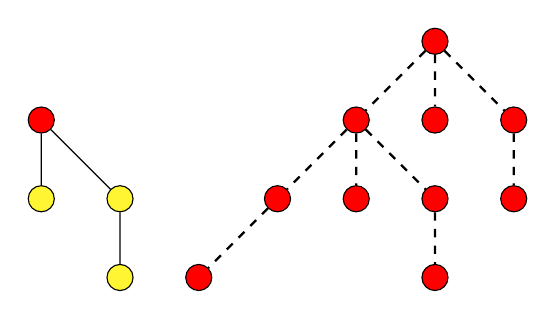
\begin{tikzpicture}
        \node[circle, draw, fill=red] (a) at (0, 0) {};
        \node[circle, draw, fill=yellow!80] (b) at (0, -1) {};
        \node[circle, draw, fill=yellow!80] (c) at (1, -1) {};
        \node[circle, draw, fill=yellow!80] (d) at (1, -2) {};
        
        \draw (a) to (b)
            (a) to (c)
            (c) to (d);
        
        \node[circle, draw, fill=red] (e) at (5, 1) {};
        \node[circle, draw, fill=red] (f) at (4, 0) {};
        \node[circle, draw, fill=red] (g) at (5, 0) {};
        \node[circle, draw, fill=red] (h) at (6, 0) {};
        \node[circle, draw, fill=red] (i) at (3, -1) {};
        \node[circle, draw, fill=red] (j) at (4, -1) {};
        \node[circle, draw, fill=red] (k) at (5, -1) {};
        \node[circle, draw, fill=red] (l) at (6, -1) {};
        \node[circle, draw, fill=red] (m) at (2, -2) {};
        \node[circle, draw, fill=red] (n) at (5, -2) {};
        
        \draw[thick, dashed] (e) to (f)
            (e) to (g)
            (e) to (h)
            (f) to (i)
            (f) to (j)
            (f) to (k)
            (h) to (l)
            (i) to (m)
            (k) to (n);
    \end{tikzpicture}
\end{figure}
\noindent We continue this process and find all the vertices like above.
\begin{figure}[H]
    \centering
    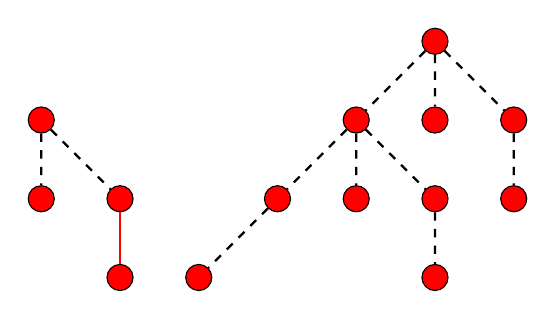
\begin{tikzpicture}
        \node[circle, draw, fill=red] (a) at (0, 0) {};
        \node[circle, draw, fill=red] (b) at (0, -1) {};
        \node[circle, draw, fill=red] (c) at (1, -1) {};
        \node[circle, draw, fill=red] (d) at (1, -2) {};
        
        \draw[thick, dashed] (a) to (b)
            (a) to (c);
        \draw[red, thick] (c) to (d);
        
        \node[circle, draw, fill=red] (e) at (5, 1) {};
        \node[circle, draw, fill=red] (f) at (4, 0) {};
        \node[circle, draw, fill=red] (g) at (5, 0) {};
        \node[circle, draw, fill=red] (h) at (6, 0) {};
        \node[circle, draw, fill=red] (i) at (3, -1) {};
        \node[circle, draw, fill=red] (j) at (4, -1) {};
        \node[circle, draw, fill=red] (k) at (5, -1) {};
        \node[circle, draw, fill=red] (l) at (6, -1) {};
        \node[circle, draw, fill=red] (m) at (2, -2) {};
        \node[circle, draw, fill=red] (n) at (5, -2) {};
        
        \draw[thick, dashed] (e) to (f)
            (e) to (g)
            (e) to (h)
            (f) to (i)
            (f) to (j)
            (f) to (k)
            (h) to (l)
            (i) to (m)
            (k) to (n);
    \end{tikzpicture}
\end{figure}
\noindent Like in the case of a depth-first search, the edges traversed in breadth-first search form a spanning tree (or a forest). We illustrate this with an example- we will traverse the following graph using breadth-first search.
\begin{figure}[H]
    \centering
    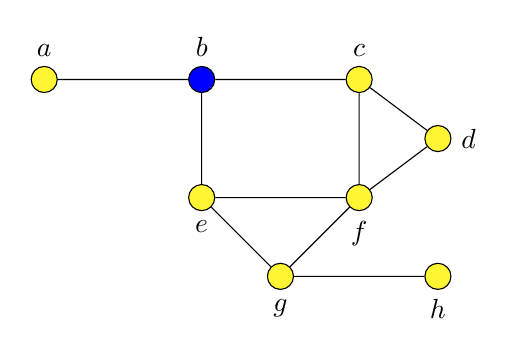
\begin{tikzpicture}
        \node[circle, draw, fill=yellow!80, label={90:$a$}] (a) at (0, -.5) {};
        \node[circle, draw, fill=blue, label={90:$b$}] (b) at (2, -.5) {};
        \node[circle, draw, fill=yellow!80, label={90:$c$}] (c) at (4, -.5) {};
        \node[circle, draw, fill=yellow!80, label={0:$d$}] (d) at (5, -1.25) {};
        \node[circle, draw, fill=yellow!80, label={-90:$e$}] (e) at (2, -2) {};
        \node[circle, draw, fill=yellow!80, label={-90:$f$}] (f) at (4, -2) {};
        \node[circle, draw, fill=yellow!80, label={-90:$g$}] (g) at (3, -3) {};
        \node[circle, draw, fill=yellow!80, label={-90:$h$}] (h) at (5, -3) {};
        
        \draw (a) to (b)
            (b) to (c)
            (c) to (d)
            (c) to (f)
            (d) to (f)
            (b) to (e)
            (e) to (f)
            (e) to (g)
            (f) to (g)
            (g) to (h);
    \end{tikzpicture}
    \caption{An undirected graph being visited by breadth-first search.}
\end{figure}
\noindent The vertices in blue are the visited vertices. At this point, the queue is $\langle b \rangle$. So, we remove $b$ from the queue and visit it.
\begin{figure}[H]
    \centering
    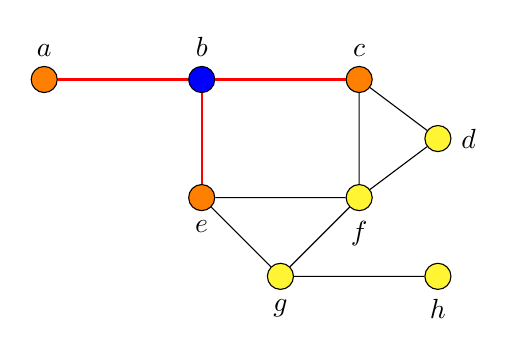
\begin{tikzpicture}
        \node[circle, draw, fill=orange, label={90:$a$}] (a) at (0, -.5) {};
        \node[circle, draw, fill=blue, label={90:$b$}] (b) at (2, -.5) {};
        \node[circle, draw, fill=orange, label={90:$c$}] (c) at (4, -.5) {};
        \node[circle, draw, fill=yellow!80, label={0:$d$}] (d) at (5, -1.25) {};
        \node[circle, draw, fill=orange, label={-90:$e$}] (e) at (2, -2) {};
        \node[circle, draw, fill=yellow!80, label={-90:$f$}] (f) at (4, -2) {};
        \node[circle, draw, fill=yellow!80, label={-90:$g$}] (g) at (3, -3) {};
        \node[circle, draw, fill=yellow!80, label={-90:$h$}] (h) at (5, -3) {};
        
        \draw[red, thick] (a) to (b)
            (b) to (c)
            (b) to (e);
        
        \draw (c) to (d)
            (c) to (f)
            (d) to (f)
            (e) to (f)
            (e) to (g)
            (f) to (g)
            (g) to (h);
    \end{tikzpicture}
\end{figure}
\noindent The vertices in orange and the edges in red are those in the queue. At this point, the queue is $\langle a, c, e \rangle$. So, we remove $a$ from the queue and visit it.
\begin{figure}[H]
    \centering
    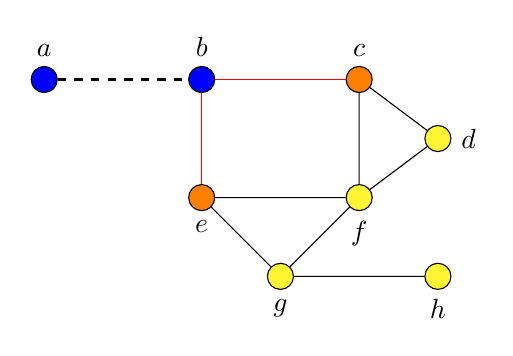
\begin{tikzpicture}
        \node[circle, draw, fill=blue, label={90:$a$}] (a) at (0, -.5) {};
        \node[circle, draw, fill=blue, label={90:$b$}] (b) at (2, -.5) {};
        \node[circle, draw, fill=orange, label={90:$c$}] (c) at (4, -.5) {};
        \node[circle, draw, fill=yellow!80, label={0:$d$}] (d) at (5, -1.25) {};
        \node[circle, draw, fill=orange, label={-90:$e$}] (e) at (2, -2) {};
        \node[circle, draw, fill=yellow!80, label={-90:$f$}] (f) at (4, -2) {};
        \node[circle, draw, fill=yellow!80, label={-90:$g$}] (g) at (3, -3) {};
        \node[circle, draw, fill=yellow!80, label={-90:$h$}] (h) at (5, -3) {};
        
        \draw[thick, dashed] (a) to (b);
        \draw[red] (b) to (c)
            (b) to (e);
        \draw (c) to (d)
            (c) to (f)
            (d) to (f)
            (e) to (f)
            (e) to (g)
            (f) to (g)
            (g) to (h);
    \end{tikzpicture}
\end{figure}
\noindent The dashed edges are the visited edges, and are therefore part of the spanning tree. We do not discover any new vertex, so the queue remains $\langle c, e \rangle$. Next, we remove $c$ from the queue and visit it.
\begin{figure}[H]
    \centering
    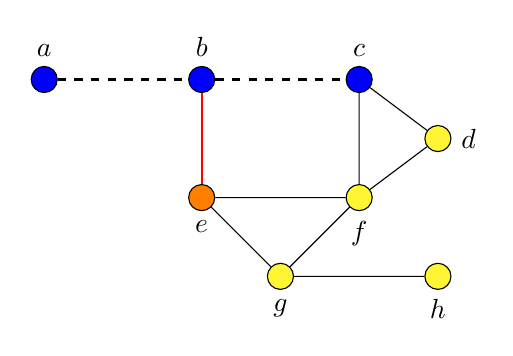
\begin{tikzpicture}
        \node[circle, draw, fill=blue, label={90:$a$}] (a) at (0, -.5) {};
        \node[circle, draw, fill=blue, label={90:$b$}] (b) at (2, -.5) {};
        \node[circle, draw, fill=blue, label={90:$c$}] (c) at (4, -.5) {};
        \node[circle, draw, fill=yellow!80, label={0:$d$}] (d) at (5, -1.25) {};
        \node[circle, draw, fill=orange, label={-90:$e$}] (e) at (2, -2) {};
        \node[circle, draw, fill=yellow!80, label={-90:$f$}] (f) at (4, -2) {};
        \node[circle, draw, fill=yellow!80, label={-90:$g$}] (g) at (3, -3) {};
        \node[circle, draw, fill=yellow!80, label={-90:$h$}] (h) at (5, -3) {};
        
        \draw[thick, dashed] (a) to (b)
            (b) to (c);
        \draw[thick, red] (b) to (e);
        \draw (c) to (d)
            (c) to (f)
            (d) to (f)
            (e) to (f)
            (e) to (g)
            (f) to (g)
            (g) to (h);
    \end{tikzpicture}
\end{figure}
\noindent We add the vertices $d$ and $f$ to the queue, and remove $e$ from the queue.
\begin{figure}[H]
    \centering
    \begin{tikzpicture}
        \node[circle, draw, fill=blue, label={90:$a$}] (a) at (0, -.5) {};
        \node[circle, draw, fill=blue, label={90:$b$}] (b) at (2, -.5) {};
        \node[circle, draw, fill=blue, label={90:$c$}] (c) at (4, -.5) {};
        \node[circle, draw, fill=orange, label={0:$d$}] (d) at (5, -1.25) {};
        \node[circle, draw, fill=blue, label={-90:$e$}] (e) at (2, -2) {};
        \node[circle, draw, fill=orange, label={-90:$f$}] (f) at (4, -2) {};
        \node[circle, draw, fill=yellow!80, label={-90:$g$}] (g) at (3, -3) {};
        \node[circle, draw, fill=yellow!80, label={-90:$h$}] (h) at (5, -3) {};
        
        \draw[dashed, thick] (a) to (b)
            (b) to (c)
            (b) to (e);
        
        \draw[red, thick] (c) to (d)
            (c) to (f);
        \draw (e) to (f)
            (d) to (f)
            (e) to (g)
            (f) to (g)
            (g) to (h);
    \end{tikzpicture}
\end{figure}
\noindent At this point, the queue is $\langle d, f \rangle$. We add $g$ to the queue, and remove $d$.
\begin{figure}[H]
    \centering
    \begin{tikzpicture}
        \node[circle, draw, fill=blue, label={90:$a$}] (a) at (0, -.5) {};
        \node[circle, draw, fill=blue, label={90:$b$}] (b) at (2, -.5) {};
        \node[circle, draw, fill=blue, label={90:$c$}] (c) at (4, -.5) {};
        \node[circle, draw, fill=blue, label={0:$d$}] (d) at (5, -1.25) {};
        \node[circle, draw, fill=blue, label={-90:$e$}] (e) at (2, -2) {};
        \node[circle, draw, fill=orange, label={-90:$f$}] (f) at (4, -2) {};
        \node[circle, draw, fill=orange, label={-90:$g$}] (g) at (3, -3) {};
        \node[circle, draw, fill=yellow!80, label={-90:$h$}] (h) at (5, -3) {};
        
        \draw[thick, dashed] (a) to (b)
            (b) to (c)
            (b) to (e)
            (c) to (d);
        \draw[red, thick] (c) to (f)
            (e) to (g);
        
        \draw (e) to (f)
            (f) to (g)
            (d) to (f)
            (g) to (h);
    \end{tikzpicture}
\end{figure}
\noindent We do not discover any new vertices, so the queue remains $\langle f, g \rangle$. So, the next vertex we visit is $f$.
\begin{figure}[H]
    \centering
    \begin{tikzpicture}
        \node[circle, draw, fill=blue, label={90:$a$}] (a) at (0, -.5) {};
        \node[circle, draw, fill=blue, label={90:$b$}] (b) at (2, -.5) {};
        \node[circle, draw, fill=blue, label={90:$c$}] (c) at (4, -.5) {};
        \node[circle, draw, fill=blue, label={0:$d$}] (d) at (5, -1.25) {};
        \node[circle, draw, fill=blue, label={-90:$e$}] (e) at (2, -2) {};
        \node[circle, draw, fill=blue, label={-90:$f$}] (f) at (4, -2) {};
        \node[circle, draw, fill=orange, label={-90:$g$}] (g) at (3, -3) {};
        \node[circle, draw, fill=yellow!80, label={-90:$h$}] (h) at (5, -3) {};
        
        \draw[thick, dashed] (a) to (b)
            (b) to (c)
            (b) to (e)
            (c) to (d)
            (c) to (f);
        
        \draw[red, thick] (e) to (g);

        \draw (e) to (f)
            (d) to (f)
            (f) to (g)
            (g) to (h);
    \end{tikzpicture}
\end{figure}
\noindent Still, we do not find any new vertex, so the queue remains $\langle g \rangle$. We then remove $g$.
\begin{figure}[H]
    \centering
    \begin{tikzpicture}
        \node[circle, draw, fill=blue, label={90:$a$}] (a) at (0, -.5) {};
        \node[circle, draw, fill=blue, label={90:$b$}] (b) at (2, -.5) {};
        \node[circle, draw, fill=blue, label={90:$c$}] (c) at (4, -.5) {};
        \node[circle, draw, fill=blue, label={0:$d$}] (d) at (5, -1.25) {};
        \node[circle, draw, fill=blue, label={-90:$e$}] (e) at (2, -2) {};
        \node[circle, draw, fill=blue, label={-90:$f$}] (f) at (4, -2) {};
        \node[circle, draw, fill=blue, label={-90:$g$}] (g) at (3, -3) {};
        \node[circle, draw, fill=orange, label={-90:$h$}] (h) at (5, -3) {};
        
        \draw[thick, dashed] (a) to (b)
            (b) to (c)
            (b) to (e)
            (c) to (d)
            (c) to (f)
            (e) to (g);
        \draw[thick, red] (g) to (h);
        \draw (e) to (f)
            (d) to (f)
            (f) to (g);
    \end{tikzpicture}
\end{figure}
\noindent Now, we find $h$, so the queue becomes $\langle h \rangle$. We visit $h$ next.
\begin{figure}[H]
    \centering
    \begin{tikzpicture}
        \node[circle, draw, fill=blue, label={90:$a$}] (a) at (0, -.5) {};
        \node[circle, draw, fill=blue, label={90:$b$}] (b) at (2, -.5) {};
        \node[circle, draw, fill=blue, label={90:$c$}] (c) at (4, -.5) {};
        \node[circle, draw, fill=blue, label={0:$d$}] (d) at (5, -1.25) {};
        \node[circle, draw, fill=blue, label={-90:$e$}] (e) at (2, -2) {};
        \node[circle, draw, fill=blue, label={-90:$f$}] (f) at (4, -2) {};
        \node[circle, draw, fill=blue, label={-90:$g$}] (g) at (3, -3) {};
        \node[circle, draw, fill=blue, label={-90:$h$}] (h) at (5, -3) {};
        
        \draw[thick, dashed] (a) to (b)
            (b) to (c)
            (b) to (e)
            (c) to (d)
            (c) to (f)
            (e) to (g)
            (g) to (h);
        \draw (e) to (f)
            (d) to (f)
            (f) to (g);
    \end{tikzpicture}
\end{figure}
\noindent We do not find any new vertex, so $h$ is visited as well. We have now finished the traversal. The dashed edges are part of the spanning tree, which is shown below.
\begin{figure}[H]
    \centering
    \begin{tikzpicture}
        \node[circle, draw, fill=yellow!80] (a) at (0, -.5) {};
        \node[circle, draw, fill=yellow!80] (b) at (2, -.5) {};
        \node[circle, draw, fill=yellow!80] (c) at (4, -.5) {};
        \node[circle, draw, fill=yellow!80] (d) at (5, -1.25) {};
        \node[circle, draw, fill=yellow!80] (e) at (2, -2) {};
        \node[circle, draw, fill=yellow!80] (f) at (4, -2) {};
        \node[circle, draw, fill=yellow!80] (g) at (3, -3) {};
        \node[circle, draw, fill=yellow!80] (h) at (5, -3) {};
        
        \draw (a) to (b)
            (b) to (c)
            (b) to (e)
            (c) to (d)
            (c) to (f)
            (g) to (h)
            (e) to (g);
    \end{tikzpicture}
    \caption{A spanning tree of the graph above, found using breadth-first search.}
\end{figure}
The following is the implementation of breadth first search using adjacency lists. It features all the code we had in order to implement adjacency lists as well.
\lstinputlisting[language=pseudocode]{src/breadthFirstSearch.psc}

We now consider the complexity of breadth-first search using adjacency lists. We visit every vertex and queue it exactly once. Also, the adjacency list is also traversed once. Therefore, the overall complexity is $O(|V| + |E|)$ using an adjacency list. If we instead used an adjacency matrix, the complexity is $O(|V|^2)$.

An application of breadth-first search to find the distance between two vertices. The distance is the number of edges in the shortest path between the two vertices. We can assign the distance from a vertex to itself as 0. Then, we can carry out a breadth-first search from the vertex, incrementing distance by 1 as we find a new vertex. We stop when we have reached the other vertex. 

We illustrate this by an example. We are finding the shortest distance/path from $b$ to $h$.
\begin{figure}[H]
    \centering
    \begin{tikzpicture}[minimum size=20pt]
        \node[circle, draw, fill=yellow!80] (a) at (0, -.5) {$a$};
        \node[circle, draw, fill=red!50] (b) at (2, -.5) {$b$};
        \node[circle, draw, fill=yellow!80] (c) at (4, -.5) {$c$};
        \node[circle, draw, fill=yellow!80] (d) at (5, -1.25) {$d$};
        \node[circle, draw, fill=yellow!80] (e) at (2, -2) {$e$};
        \node[circle, draw, fill=yellow!80] (f) at (4, -2) {$f$};
        \node[circle, draw, fill=yellow!80] (g) at (3, -3) {$g$};
        \node[circle, draw, fill=blue!50] (h) at (5, -3) {$h$};
        
        \draw (a) to (b)
            (b) to (c)
            (c) to (d)
            (c) to (f)
            (d) to (f)
            (b) to (e)
            (e) to (f)
            (e) to (g)
            (f) to (g)
            (g) to (h);
    \end{tikzpicture}
    \caption{An undirected graph, where we want to find the distance between the vertices $b$ and $h$.}
\end{figure}
\noindent From $b$, we find three vertices- $a$, $c$ and $e$. We assign these three vertices distance 1 and add them to the queue. The queue is therefore $\langle a, c, e \rangle$.
\begin{figure}[H]
    \centering
    \begin{tikzpicture}[minimum size=20pt]
        \node[circle, draw, fill=orange!50, label={180:1}] (a) at (0, -.5) {$a$};
        \node[circle, draw, fill=red!50] (b) at (2, -.5) {$b$};
        \node[circle, draw, fill=orange!50, label={0:1}] (c) at (4, -.5) {$c$};
        \node[circle, draw, fill=yellow!80] (d) at (5, -1.25) {$d$};
        \node[circle, draw, fill=orange!50, label={180:1}] (e) at (2, -2) {$e$};
        \node[circle, draw, fill=yellow!80] (f) at (4, -2) {$f$};
        \node[circle, draw, fill=yellow!80] (g) at (3, -3) {$g$};
        \node[circle, draw, fill=blue!50] (h) at (5, -3) {$h$};
        
        \draw[thick, dashed] (b) to (a)
            (b) to (c)
            (b) to (e);
        \draw (c) to (d)
            (c) to (f)
            (d) to (f)
            (e) to (f)
            (e) to (g)
            (f) to (g)
            (g) to (h);
    \end{tikzpicture}
\end{figure}
\noindent The dotted lines represent the shortest path we can take from a vertex to $b$, and the orange vertices are those for which we know the shortest path. The queue is $\langle a, c, e \rangle$. So, we first pop $a$. We do not discover any more vertices from $a$- the queue remains $\langle c, e \rangle$. Next, we pop $c$ and find the vertices $d$ and $f$. These vertices have distance 2, and the queue is now $\langle e, d, f \rangle$.
\begin{figure}[H]
    \centering
    \begin{tikzpicture}[minimum size=20pt]
        \node[circle, draw, fill=orange!50, label={180:1}] (a) at (0, -.5) {$a$};
        \node[circle, draw, fill=red!50] (b) at (2, -.5) {$b$};
        \node[circle, draw, fill=orange!50, label={0:1}] (c) at (4, -.5) {$c$};
        \node[circle, draw, fill=orange!50, label={45:2}] (d) at (5, -1.25) {$d$};
        \node[circle, draw, fill=orange!50, label={180:1}] (e) at (2, -2) {$e$};
        \node[circle, draw, fill=orange!50, label={0:2}] (f) at (4, -2) {$f$};
        \node[circle, draw, fill=yellow!80] (g) at (3, -3) {$g$};
        \node[circle, draw, fill=blue!50] (h) at (5, -3) {$h$};
        
        \draw[thick, dashed] (b) to (a)
            (b) to (c)
            (b) to (e)
            (c) to (d)
            (c) to (f);
        \draw (d) to (f)
            (e) to (f)
            (e) to (g)
            (f) to (g)
            (g) to (h);
    \end{tikzpicture}
\end{figure}
\noindent From the queue, we pop $e$. We then discover the vertex $g$. This vertex has distance 2, and the queue is now $\langle d, f, g \rangle$. We process $e$ before $f$ since $f$ was added to the queue later- that is why $g$ gets assigned distance 2 (correctly), and not 3. 
\begin{figure}[H]
    \centering
    \begin{tikzpicture}[minimum size=20pt]
        \node[circle, draw, fill=orange!50, label={180:1}] (a) at (0, -.5) {$a$};
        \node[circle, draw, fill=red!50] (b) at (2, -.5) {$b$};
        \node[circle, draw, fill=orange!50, label={0:1}] (c) at (4, -.5) {$c$};
        \node[circle, draw, fill=orange!50, label={45:2}] (d) at (5, -1.25) {$d$};
        \node[circle, draw, fill=orange!50, label={180:1}] (e) at (2, -2) {$e$};
        \node[circle, draw, fill=orange!50, label={0:2}] (f) at (4, -2) {$f$};
        \node[circle, draw, fill=orange!50, label={180:2}] (g) at (3, -3) {$g$};
        \node[circle, draw, fill=blue!50] (h) at (5, -3) {$h$};
        
        \draw[thick, dashed] (b) to (a)
            (b) to (c)
            (b) to (e)
            (c) to (d)
            (c) to (f)
            (e) to (g);
        \draw (d) to (f) 
            (e) to (f)
            (f) to (g)
            (g) to (h);
    \end{tikzpicture}
\end{figure}
\noindent Next, we pop the vertices $d$ and $f$ from the queue. They are not incident to any unvisited vertices, so after popping, the queue is $\langle g \rangle$. Then, we visit the vertex $g$. We can finally assign distance to the vertex $h$- it is 3.
\begin{figure}[H]
    \centering
    \begin{tikzpicture}[minimum size=20pt]
        \node[circle, draw, fill=orange!50, label={180:1}] (a) at (0, -.5) {$a$};
        \node[circle, draw, fill=red!50] (b) at (2, -.5) {$b$};
        \node[circle, draw, fill=orange!50, label={0:1}] (c) at (4, -.5) {$c$};
        \node[circle, draw, fill=orange!50, label={45:2}] (d) at (5, -1.25) {$d$};
        \node[circle, draw, fill=orange!50, label={180:1}] (e) at (2, -2) {$e$};
        \node[circle, draw, fill=orange!50, label={0:2}] (f) at (4, -2) {$f$};
        \node[circle, draw, fill=orange!50, label={180:2}] (g) at (3, -3) {$g$};
        \node[circle, draw, fill=blue!50, label={0:3}] (h) at (5, -3) {$h$};
        
        \draw[thick, dashed] (b) to (a)
            (b) to (c)
            (b) to (e)
            (c) to (d)
            (c) to (f)
            (e) to (g)
            (g) to (h);
        \draw (d) to (f) 
            (e) to (f)
            (f) to (g);
    \end{tikzpicture}
\end{figure}
\noindent The algorithm has now terminated. The shortest distance between $b$ and $h$ has been correctly computed to be 3. We can also find the shortest path by following the dashed edges from $h$.
\newpage

\section{Weighted Graphs}
In a weighted graph, each edge has a weight that is strictly positive. The graph can be both directed or undirected. The weight may represent length, cost, capacity, etc. If an edge is not part of the graph, we assume that its weight is infinity.

An example of a weighted graph is given below.
\begin{figure}[H]
    \centering
    \begin{tikzpicture}
        \node[circle, draw] (u) at (0, 0) {$u$};
        \node[circle, draw] (v) at (-2, -.75) {$v$};
        \node[circle, draw] (w) at (2, -.75) {$w$};
        \node[circle, draw] (x) at (-2, -2.25) {$x$};
        \node[circle, draw] (y) at (2, -2.25) {$y$};
        \node[circle, draw] (z) at (0, -3) {$z$};
        
        \draw (u) to node[above left] {4} (v)
            (u) to node[above right] {5} (w)
            (w) to node[right] {4} (y)
            (y) to node[below right] {7} (z)
            (x) to node[below left] {6} (z)
            (x) to node[left] {6} (v)
            (x) to node[below right] {7} (u)
            (z) to node[above left] {5} (w)
            (v) to node[above] {5} (w)
            (x) to node[below] {8} (y);
    \end{tikzpicture}
    \caption{A weighted graph.}
\end{figure}
We can represent a weighted graph as both adjacency matrix and adjacency list. An adjacency matrix becomes the weight matrix, while an adjacency list stores the weight within the array, as a tuple corresponding to a particular edge. 

So, the weighted graph above can be represented as follows.
\begin{table}[H]
    \centering
    \begin{tabular}{c|cccccc}
         & $u$ & $v$ & $w$ & $x$ & $y$ & $z$ \\
         \hline
        $u$ & 0 & 4 & 5 & 7 & 0 & 0 \\
        $v$ & 4 & 0 & 5 & 6 & 0 & 0 \\
        $w$ & 5 & 5 & 0 & 0 & 4 & 5 \\
        $x$ & 7 & 6 & 0 & 0 & 8 & 6 \\
        $y$ & 0 & 0 & 4 & 8 & 0 & 7 \\
        $z$ & 0 & 0 & 5 & 6 & 7 & 0
    \end{tabular}
    \caption{The adjacency matrix representation of the weighted graph above}
\end{table}
\noindent Moreover, the adjacency list is given below.
\begin{table}[H]
    \centering
    \begin{tabular}{c|l}
        $u$ & $[(v, 4), (w, 5), (x, 7)]$ \\
        $v$ & $[(u, 4), (w, 5), (x, 6)]$\\
        $w$ & $[(u, 5), (v, 5), (y, 4), (z, 5)]$ \\
        $x$ & $[(u, 7), (v, 6), (y, 8), (z, 6)]$\\
        $y$ & $[(w, 4), (x, 8), (z, 7)]$ \\
        $z$ & $[(w, 5), (x, 6), (y, 7)]$
    \end{tabular}
    \caption{The adjacency list representation for the weighted graph above}
\end{table}
\subsection{Shortest Path}
Given a weighted graph and two vertices $u$ and $v$, the shortest path algorithm computes the shortest path between $u$ and $v$ with respect to their weight. We say that the length of the path is the sum of the weights of its edges.

Dijkstra's algorithm finds the shortest path between a vertex $u$ and all the other vertices. It is based on maintaining a set $S$ containing all the vertices for which the shortest path with $u$ is currently known. Initially, $S$ only contains the vertex $u$. Eventually, $S$ contains all the vertices, i.e. the shortest path to all the vertices from $u$ is known. 

Each vertex $v$ has a label $d(v)$ indicating the length of the shortest path between $u$ and $v$, passing only through the vertices in $S$. $S$ gets updated as the algorithm runs, so we change $d(v)$ as we add more elements. If there is no path, we set $d(v)$ to infinity. If $v$ is in $S$, then $d(v)$ is the length of the shortest path between $u$ and $v$. 

If $v$ is in $S$ and $w$ is not in $S$, then we want the length of the shortest path between $u$ and $w$ to be at least that between $u$ and $v$. Otherwise, the distance between $u$ and $w$ would be smaller. In that case, there would be an edge connecting $w$ to a vertex in $S$ with a smaller weight than the one connecting $v$ to another vertex in $S$. We don't want this because it might be possible to improve the distance between $u$ and $v$ using this edge. Therefore, we need to ensure that the vertex we add to $S$ during each iteration has the smallest weight so that a vertex not in $S$ cannot be used to find a shorter distance between $u$ and a vertex in $S$.
% TODO: Add pictures to represent this?

In Dijkstra's algorithm, we add to $S$ the vertex $v$ not in $S$ such that $d(v)$ is minimum among those not in $S$. As explained above, this ensures that the shortest path for vertices not in $S$ to $u$ have length greater than or equal to that for all vertices in $S$.

After adding a vertex $v$ to $S$, we carry out \emph{edge relaxation} operations. This means we update the length $d(w)$ for all vertices $w$ that are still not in $S$. We previously have computed $d(w)$ based on all the vertices in $S$. We have added a $v$ to $S$, so we might need to update the shortest distance if there is a better edge from $v$ to $w$. In fact, the updated distance is given by
\[d(w) = \min(d(w), d(v) + wt(e)),\]
where $wt(e)$ is the weight of the edge $e$ that is incident to the new vertex $v$.

Using this formula, we can construct the pseudocode for the Dijkstra's algorithm.
\lstinputlisting[language=pseudocode]{src/dijkstra.psc}
The function \texttt{\_minVertex} finds the vertex not in $S$ such that the edge from the vertex to some vertex in $S$ has the minimum weight.

We will now analyse the algorithm. Assume that we have $n$ vertices and $m$ edges. Using an unordered array to store the lengths, it takes $O(n)$ to initialise the lengths. Finding the minimum vertex is $O(n^2)$ overall- each time, it takes $O(n)$ to find the minimum, and we find it $n-1$ times. The relaxation is $O(m)$ overall- each edge is considered once, and updating the length takes $O(1)$. Therefore, the complexity of Dijkstra's algorithm is $O(n^2 + m)$. Since the number of edges is at most $n(n-1)$, this is equivalent to $O(n^2)$.

Instead of using an unordered array, we can use a heap to store the lengths. In that case, it still takes $O(n)$ to initialise the lengths and create a heap. Finding the minimum is now $O(n \log n)$- each time, it takes $O(\log n)$ to find the minimum, and we find it $n-1$ times. The relaxation is $O(m \log n)$ overall- each edge is considered once, and the updating takes $O(\log n)$. This updates a certain value in the heap (not necessarily the root). We would also need to keep track of each vertex distance in the heap, so care must be taken. Therefore, the complexity is $O((m+n) \log n)$. Assuming a graph has more edges than vertices, we can simplify the complexity to $O(m \log n)$. A graph with $n$ vertices could have $O(n^2)$ edges, so the complexity may be $O(n^2 \log n)$- this is not better than $O(n^2)$ using an unordered array.

We shall now illustrate Dijkstra's algorithm with an example. The graph below is a directed weighted graph, and we aim to find the minimum distance from $u$.
\begin{figure}[H]
    \centering
    \begin{tikzpicture}
        \node[circle, draw=red, fill=yellow!80, label={180:0}, text=red] (u) at (0, 0) {$u$};
        \node[circle, draw, fill=yellow!80] (v) at (1, 1) {$v$};
        \node[circle, draw, fill=yellow!80] (w) at (1, -1) {$w$};
        \node[circle, draw, fill=yellow!80] (x) at (3, 1) {$x$};
        \node[circle, draw, fill=yellow!80] (y) at (3, -1) {$y$};
        \node[circle, draw, fill=yellow!80] (z) at (4, 0) {$z$};
        
        \draw[->] (u) -- node[above] {2} (v);
        \draw[->] (v) -- node[above] {4} (x);
        \draw[->] (x) -- node[above] {6} (z);
        \draw[->] (y) -- node[below] {4} (z);
        \draw[->] (w) -- node[below] {7} (y);
        \draw[->] (u) -- node[below] {8} (w);
        \draw[->] (v) -- node[left] {3} (w);
        \draw[->] (w) -- node[below right, pos=0.8] {2} (x);
        \draw[->] (x) -- node[right] {1} (y);
        \draw[->] (v) -- node[above right, pos=0.2] {9} (y);
    \end{tikzpicture}
    \caption{A weighted graph whose distances (from $u$) are to be found using Dijkstra's algorithm.}
\end{figure}
\noindent Vertices whose shortest path to $u$ is known are labelled with red text. First, we set the distance of $u$ from $u$ to be 0. Any distance we do not know is $\infty$. Considering vertices going from $S = \{u\}$ to those not in $S$, we choose the edge connected with the smallest distance- it is $u \to v$. So, we add $v$ to $S$.
\begin{figure}[H]
    \centering
    \begin{tikzpicture}
        \node[circle, draw=red, fill=yellow!80, label={180:0}, text=red] (u) at (0, 0) {$u$};
        \node[circle, draw=red, fill=yellow!80, label={90:2}, text=red] (v) at (1, 1) {$v$};
        \node[circle, draw=red, fill=yellow!80, label={-90:8}] (w) at (1, -1) {$w$};
        \node[circle, draw, fill=yellow!80] (x) at (3, 1) {$x$};
        \node[circle, draw, fill=yellow!80] (y) at (3, -1) {$y$};
        \node[circle, draw, fill=yellow!80] (z) at (4, 0) {$z$};
        
        \draw[->, thick, dashed, dashed] (u) -- node[above] {2} (v);
        \draw[->] (v) -- node[above] {4} (x);
        \draw[->] (x) -- node[above] {6} (z);
        \draw[->] (y) -- node[below] {4} (z);
        \draw[->] (w) -- node[below] {7} (y);
        \draw[->, thick, dashed, dashed] (u) -- node[below] {8} (w);
        \draw[->] (v) -- node[left] {3} (w);
        \draw[->] (w) -- node[below right, pos=0.8] {2} (x);
        \draw[->] (x) -- node[right] {1} (y);
        \draw[->] (v) -- node[above right, pos=0.2] {9} (y);
    \end{tikzpicture}
\end{figure}
\noindent Vertices for which we know a path (not necessarily the shortest path) from $u$ are shown with a red border. Dashed edges represent the path from $u$ to that vertex, if known. At this point, $S = \{u, v\}$. We relax the edges with respect to the vertex $v$.
\begin{figure}[H]
    \centering
    \begin{tikzpicture}
        \node[circle, draw=red, fill=yellow!80, label={180:0}, text=red] (u) at (0, 0) {$u$};
        \node[circle, draw=red, fill=yellow!80, label={90:2}, text=red] (v) at (1, 1) {$v$};
        \node[circle, draw=red, fill=yellow!80, label={-90:5}, text=red] (w) at (1, -1) {$w$};
        \node[circle, draw=red, fill=yellow!80, label={90:6}] (x) at (3, 1) {$x$};
        \node[circle, draw=red, fill=yellow!80, label={-90:11}] (y) at (3, -1) {$y$};
        \node[circle, draw, fill=yellow!80] (z) at (4, 0) {$z$};
        
        \draw[->, thick, dashed] (u) -- node[above] {2} (v);
        \draw[->, thick, dashed] (v) -- node[above] {4} (x);
        \draw[->] (x) -- node[above] {6} (z);
        \draw[->] (y) -- node[below] {4} (z);
        \draw[->] (w) -- node[below] {7} (y);
        \draw[->] (u) -- node[below] {8} (w);
        \draw[->, thick, dashed] (v) -- node[left] {3} (w);
        \draw[->] (w) -- node[below right, pos=0.8] {2} (x);
        \draw[->] (x) -- node[right] {1} (y);
        \draw[->, thick, dashed] (v) -- node[above right, pos=0.2] {9} (y);
    \end{tikzpicture}
\end{figure}
\noindent Now, we know the distance from $u$ to $x$ and $y$. Also, we have found a shorter distance from $u$ to $w$, going through $v$. The edge with smallest weight from a vertex not in $S$ to a vertex in $S$ is $v \to w$, so we add $w$ to $S$. We then relax the vertices with respect to $w$.
\begin{figure}[H]
    \centering
    \begin{tikzpicture}
        \node[circle, draw=red, fill=yellow!80, label={180:0}, text=red] (u) at (0, 0) {$u$};
        \node[circle, draw=red, fill=yellow!80, label={90:2}, text=red] (v) at (1, 1) {$v$};
        \node[circle, draw=red, fill=yellow!80, label={-90:5}, text=red] (w) at (1, -1) {$w$};
        \node[circle, draw=red, fill=yellow!80, label={90:6}, text=red] (x) at (3, 1) {$x$};
        \node[circle, draw=red, fill=yellow!80, label={-90:11}] (y) at (3, -1) {$y$};
        \node[circle, draw, fill=yellow!80] (z) at (4, 0) {$z$};
        
        \draw[->, thick, dashed] (u) -- node[above] {2} (v);
        \draw[->, thick, dashed] (v) -- node[above] {4} (x);
        \draw[->] (x) -- node[above] {6} (z);
        \draw[->] (y) -- node[below] {4} (z);
        \draw[->] (w) -- node[below] {7} (y);
        \draw[->] (u) -- node[below] {8} (w);
        \draw[->, thick, dashed] (v) -- node[left] {3} (w);
        \draw[->] (w) -- node[below right, pos=0.8] {2} (x);
        \draw[->] (x) -- node[right] {1} (y);
        \draw[->, thick, dashed] (v) -- node[above right, pos=0.2] {9} (y);
    \end{tikzpicture}
\end{figure}
\noindent We do not change any path since going through $w$ only increases the weight. Also, we do not discover the distance to $z$. Here, the smallest-weighted edge is $v \to x$. So, we add $x$ to $S$ and relax the vertices with respect to $x$.
\begin{figure}[H]
    \centering
    \begin{tikzpicture}
        \node[circle, draw=red, fill=yellow!80, label={180:0}, text=red] (u) at (0, 0) {$u$};
        \node[circle, draw=red, fill=yellow!80, label={90:2}, text=red] (v) at (1, 1) {$v$};
        \node[circle, draw=red, fill=yellow!80, label={-90:5}, text=red] (w) at (1, -1) {$w$};
        \node[circle, draw=red, fill=yellow!80, label={90:6}, text=red] (x) at (3, 1) {$x$};
        \node[circle, draw=red, fill=yellow!80, label={-90:7}, text=red] (y) at (3, -1) {$y$};
        \node[circle, draw=red, fill=yellow!80, label={0:12}] (z) at (4, 0) {$z$};
        
        \draw[->, thick, dashed] (u) -- node[above] {2} (v);
        \draw[->, thick, dashed] (v) -- node[above] {4} (x);
        \draw[->, thick, dashed] (x) -- node[above] {6} (z);
        \draw[->] (y) -- node[below] {4} (z);
        \draw[->] (w) -- node[below] {7} (y);
        \draw[->] (u) -- node[below] {8} (w);
        \draw[->, thick, dashed] (v) -- node[left] {3} (w);
        \draw[->] (w) -- node[below right, pos=0.8] {2} (x);
        \draw[->, thick, dashed] (x) -- node[right] {1} (y);
        \draw[->] (v) -- node[above right, pos=0.2] {9} (y);
    \end{tikzpicture}
\end{figure}
\noindent We can find a path with smaller weight from $x$ to $y$, and we have finally found a non-infinite distance from $u$ to $z$. Now, the smallest weighted edge is $x \to y$. So, we add $y$ to $S$ and relax the edges with respect to $y$.
\begin{figure}[H]
    \centering
    \begin{tikzpicture}
        \node[circle, draw=red, fill=yellow!80, label={180:0}, text=red] (u) at (0, 0) {$u$};
        \node[circle, draw=red, fill=yellow!80, label={90:2}, text=red] (v) at (1, 1) {$v$};
        \node[circle, draw=red, fill=yellow!80, label={-90:5}, text=red] (w) at (1, -1) {$w$};
        \node[circle, draw=red, fill=yellow!80, label={90:6}, text=red] (x) at (3, 1) {$x$};
        \node[circle, draw=red, fill=yellow!80, label={-90:7}, text=red] (y) at (3, -1) {$y$};
        \node[circle, draw=red, fill=yellow!80, label={0:11}, text=red] (z) at (4, 0) {$z$};
        
        \draw[->, thick, dashed] (u) -- node[above] {2} (v);
        \draw[->, thick, dashed] (v) -- node[above] {4} (x);
        \draw[->] (x) -- node[above] {6} (z);
        \draw[->, thick, dashed] (y) -- node[below] {4} (z);
        \draw[->] (w) -- node[below] {7} (y);
        \draw[->] (u) -- node[below] {8} (w);
        \draw[->, thick, dashed] (v) -- node[left] {3} (w);
        \draw[->] (w) -- node[below right, pos=0.8] {2} (x);
        \draw[->, thick, dashed] (x) -- node[right] {1} (y);
        \draw[->] (v) -- node[above right, pos=0.2] {9} (y);
    \end{tikzpicture}
\end{figure}
\noindent At this point, the only weight we can change is of $z$. It turns out that the weight going through $y$ is smaller, so we change that weight. There is only one element not in $S$, so we add it into $S$ via the edge $y$ to $z$. All the edges are now in $S$, so the algorithm terminates. We have found the shortest distance and the path going from $u$ to a particular vertex. Also, we can use the dashed arrows to follow this optimal path from a vertex to $u$.

We illustrate another example for unweighted graphs. We will find the distance from $u$ to every vertex.
\begin{figure}[H]
    \centering
    \begin{tikzpicture}
        \node[circle, draw=red, fill=yellow!80, text=red, label={90:0}] (u) at (0, 1) {$u$};
        \node[circle, draw, fill=yellow!80] (v) at (-2, -.5) {$v$};
        \node[circle, draw, fill=yellow!80] (w) at (0, -.5) {$w$};
        \node[circle, draw, fill=yellow!80] (x) at (2, -.5) {$x$};
        \node[circle, draw, fill=yellow!80] (y) at (-1, -2) {$y$};
        \node[circle, draw, fill=yellow!80] (z) at (1, -2) {$z$};
        
        \draw (u) -- node[above left] {8} (v)
            (u) -- node[above right] {4} (x)
            (u) -- node[right] {2} (w)
            (v) -- node[right] {2} (y)
            (v) -- node[above] {7} (w)
            (w) -- node[above] {1} (x)
            (w) -- node[right] {9} (z)
            (x) -- node[left] {5} (z)
            (w) -- node[left] {3} (y);
    \end{tikzpicture}
    \caption{A weighted graph whose distances (from $u$) are to be found using Dijkstra's algorithm.}
\end{figure}
\noindent Vertices whose shortest path to $u$ is known are labelled with red text. At the start, we only know the distance from $u$ to $u$- it is 0. We relax the edges with respect to $u$ to find the distance from $u$ to the other vertices.
\begin{figure}[H]
    \centering
    \begin{tikzpicture}
        \node[circle, draw=red, fill=yellow!80, text=red, label={90:0}] (u) at (0, 1) {$u$};
        \node[circle, draw=red, fill=yellow!80, label={180:8}] (v) at (-2, -.5) {$v$};
        \node[circle, draw=red, fill=yellow!80, label={-90:2}, text=red] (w) at (0, -.5) {$w$};
        \node[circle, draw=red, fill=yellow!80, label={0:4}] (x) at (2, -.5) {$x$};
        \node[circle, draw, fill=yellow!80] (y) at (-1, -2) {$y$};
        \node[circle, draw, fill=yellow!80] (z) at (1, -2) {$z$};
        
        \draw[thick, dashed] (u) -- node[above left] {8} (v)
            (u) -- node[above right] {4} (x)
            (u) -- node[right] {2} (w);
        \draw (v) -- node[right] {2} (y)
            (v) -- node[above] {7} (w)
            (w) -- node[above] {1} (x)
            (w) -- node[right] {9} (z)
            (x) -- node[left] {5} (z)
            (w) -- node[left] {3} (y);
    \end{tikzpicture}
\end{figure}
\noindent Vertices for which we know a path from $u$ are shown with a red border. Dashed edges represent the path from $u$ to that vertex, if known. The smallest-weighted vertex not in $S$ is $w$. So, we add $w$ to $S$, and relax with respect to it.

\begin{figure}[H]
    \centering
    \begin{tikzpicture}
        \node[circle, draw=red, fill=yellow!80, text=red, label={90:0}] (u) at (0, 1) {$u$};
        \node[circle, draw=red, fill=yellow!80, label={180:8}] (v) at (-2, -.5) {$v$};
        \node[circle, draw=red, fill=yellow!80, label={-90:2}, text=red] (w) at (0, -.5) {$w$};
        \node[circle, draw=red, fill=yellow!80, label={0:3}, text=red] (x) at (2, -.5) {$x$};
        \node[circle, draw=red, fill=yellow!80, label={-90:5}] (y) at (-1, -2) {$y$};
        \node[circle, draw=red, fill=yellow!80, label={-90:11}] (z) at (1, -2) {$z$};
        
        \draw[thick, dashed] (u) -- node[above left] {8} (v)
            (u) -- node[right] {2} (w)
            (w) -- node[above] {1} (x)
            (w) -- node[right] {9} (z)
            (w) -- node[left] {3} (y);
        \draw (v) -- node[right] {2} (y)
            (v) -- node[above] {7} (w)
            (u) -- node[above right] {4} (x)
            (x) -- node[left] {5} (z);
    \end{tikzpicture}
\end{figure}
\noindent We now know the distance from $u$ to $y$ and $z$. Also, the distance from $u$ to $x$ is updated- it is now 3. We did not change the distance from $u$ to $v$ because the path through $w$ is not better. Now, the smallest distance from an element not in $S$ is $x$. So, we relax the edges with respect to $x$.
\begin{figure}[H]
    \centering
    \begin{tikzpicture}
        \node[circle, draw=red, fill=yellow!80, text=red, label={90:0}] (u) at (0, 1) {$u$};
        \node[circle, draw=red, fill=yellow!80, label={180:8}] (v) at (-2, -.5) {$v$};
        \node[circle, draw=red, fill=yellow!80, label={-90:2}, text=red] (w) at (0, -.5) {$w$};
        \node[circle, draw=red, fill=yellow!80, label={0:3}, text=red] (x) at (2, -.5) {$x$};
        \node[circle, draw=red, fill=yellow!80, label={-90:5}, text=red] (y) at (-1, -2) {$y$};
        \node[circle, draw=red, fill=yellow!80, label={-90:8}] (z) at (1, -2) {$z$};
        
        \draw[thick, dashed] (u) -- node[above left] {8} (v)
            (u) -- node[right] {2} (w)
            (w) -- node[above] {1} (x)
            (w) -- node[left] {3} (y)
            (x) -- node[left] {5} (z);
        \draw (v) -- node[right] {2} (y)
            (v) -- node[above] {7} (w)
            (u) -- node[above right] {4} (x)
            (w) -- node[right] {9} (z);
    \end{tikzpicture}
\end{figure}
\noindent Following the relaxation, we have found a shorter path to $z$. Now, the smallest distance of an element not in $S$ is from $y$. So, we relax the edges with respect to $y$.
\begin{figure}[H]
    \centering
    \begin{tikzpicture}
        \node[circle, draw=red, fill=yellow!80, text=red, label={90:0}] (u) at (0, 1) {$u$};
        \node[circle, draw=red, fill=yellow!80, label={180:7}, text=red] (v) at (-2, -.5) {$v$};
        \node[circle, draw=red, fill=yellow!80, label={-90:2}, text=red] (w) at (0, -.5) {$w$};
        \node[circle, draw=red, fill=yellow!80, label={0:3}, text=red] (x) at (2, -.5) {$x$};
        \node[circle, draw=red, fill=yellow!80, label={-90:5}, text=red] (y) at (-1, -2) {$y$};
        \node[circle, draw=red, fill=yellow!80, label={-90:8}] (z) at (1, -2) {$z$};
        
        \draw[thick, dashed] (u) -- node[right] {2} (w)
            (w) -- node[above] {1} (x)
            (w) -- node[left] {3} (y)
            (x) -- node[left] {5} (z)
            (v) -- node[right] {2} (y);
        \draw (u) -- node[above left] {8} (v)
            (v) -- node[above] {7} (w)
            (u) -- node[above right] {4} (x)
            (w) -- node[right] {9} (z);
    \end{tikzpicture}
\end{figure}
\noindent We have now found a shorter path from $u$ to $v$. The next vertex to be added to $S$ is $v$. So, we relax the edges with respect to $v$.
\begin{figure}[H]
    \centering
    \begin{tikzpicture}
        \node[circle, draw=red, fill=yellow!80, text=red, label={90:0}] (u) at (0, 1) {$u$};
        \node[circle, draw=red, fill=yellow!80, label={180:7}, text=red] (v) at (-2, -.5) {$v$};
        \node[circle, draw=red, fill=yellow!80, label={-90:2}, text=red] (w) at (0, -.5) {$w$};
        \node[circle, draw=red, fill=yellow!80, label={0:3}, text=red] (x) at (2, -.5) {$x$};
        \node[circle, draw=red, fill=yellow!80, label={-90:5}, text=red] (y) at (-1, -2) {$y$};
        \node[circle, draw=red, fill=yellow!80, label={-90:8}, text=red] (z) at (1, -2) {$z$};
        
        \draw[thick, dashed] (u) -- node[right] {2} (w)
            (w) -- node[above] {1} (x)
            (w) -- node[left] {3} (y)
            (x) -- node[left] {5} (z)
            (v) -- node[right] {2} (y);
        \draw (u) -- node[above left] {8} (v)
            (v) -- node[above] {7} (w)
            (u) -- node[above right] {4} (x)
            (w) -- node[right] {9} (z);
    \end{tikzpicture}
\end{figure}
\noindent At this point, the only weight that could change is of $z$. This does not change after the relaxation. Now, we add the final vertex $z$ into $S$. We have now added all the vertices into $S$, so we have found the minimum distance from $u$ to all the vertices.
\newpage

\section{Minimum Spanning Trees}
A spanning tree is a subgraph (a subset of edges) which is both a tree and spans every vertex. It is obtained from a connected graph by deleting edges. The weight of a spanning tree is the sum of the weights of its edges. For example, in the weighted graph below, we can remove the red edges and one of the three dashed edges to get a spanning tree.
\begin{figure}[H]
    \centering
    \begin{tikzpicture}
        \node[circle, draw] (u) at (0, 0) {$u$};
        \node[circle, draw] (v) at (-1.5, -.75) {$v$};
        \node[circle, draw] (w) at (1.5, -.75) {$w$};
        \node[circle, draw] (x) at (-1.5, -2.25) {$x$};
        \node[circle, draw] (y) at (1.5, -2.25) {$y$};
        \node[circle, draw] (z) at (0, -3) {$z$};
        
        \draw[red] (u) to node[above left, text=black] {4} (v)
            (x) to node[below, text=black] {8} (y)
            (x) to node[below left, text=black] {6} (z)
            (x) to node[below right, text=black] {7} (u);
        \draw[red, dashed] (w) to node[right, text=black] {4} (y)
            (y) to node[below right, text=black] {7} (z)
            (z) to node[above left, text=black] {5} (w);
        \draw (u) to node[above right] {5} (w)
            (x) to node[left] {6} (v)
            (v) to node[above] {5} (w);
    \end{tikzpicture}
    \caption{A weighted graph whose edges are to be deleted to form a spanning tree. The red edges can be removed, and so can one of the three dashed edges.}
\end{figure}
\noindent Two of the possible spanning trees are given below.
\begin{figure}[H]
    \centering
    \begin{tikzpicture}
    \begin{scope}
        \node[circle, draw] (u) at (0, 0) {$u$};
        \node[circle, draw] (v) at (-1.5, -.75) {$v$};
        \node[circle, draw] (w) at (1.5, -.75) {$w$};
        \node[circle, draw] (x) at (-1.5, -2.25) {$x$};
        \node[circle, draw] (y) at (1.5, -2.25) {$y$};
        \node[circle, draw] (z) at (0, -3) {$z$};
        
        \draw (u) to node[above right] {5} (w)
            (x) to node[left] {6} (v)
            (v) to node[above] {5} (w)
            (z) to node[above left, text=black] {5} (w)
            (y) to node[below right] {7} (z);
    \end{scope}
    \begin{scope}
        \node[circle, draw] (u) at (5, 0) {$u$};
        \node[circle, draw] (v) at (3.5, -.75) {$v$};
        \node[circle, draw] (w) at (6.5, -.75) {$w$};
        \node[circle, draw] (x) at (3.5, -2.25) {$x$};
        \node[circle, draw] (y) at (6.5, -2.25) {$y$};
        \node[circle, draw] (z) at (5, -3) {$z$};
        
        \draw (u) to node[above right] {5} (w)
            (x) to node[left] {6} (v)
            (v) to node[above] {5} (w)
            (w) to node[right] {4} (y)
            (y) to node[below right] {7} (z);
    \end{scope}
    \end{tikzpicture}
    \caption{Two distinct spanning trees of the graph above.}
\end{figure}
\noindent The weight of the left tree is 28, while the weight of the right tree is 27. In this section, we will consider an algorithm that computes the minimum weight spanning tree. For the graph above, a minimum spanning tree is given below.
\begin{figure}[H]
    \centering
    \begin{tikzpicture}
        \node[circle, draw] (u) at (0, 0) {$u$};
        \node[circle, draw] (v) at (-1.5, -.75) {$v$};
        \node[circle, draw] (w) at (1.5, -.75) {$w$};
        \node[circle, draw] (x) at (-1.5, -2.25) {$x$};
        \node[circle, draw] (y) at (1.5, -2.25) {$y$};
        \node[circle, draw] (z) at (0, -3) {$z$};
        
        \draw (u) to node[above left] {4} (v)
            (x) to node[below left] {6} (z)
            (w) to node[right] {4} (y)
            (z) to node[above left] {5} (w)
            (u) to node[above right] {5} (w);
    \end{tikzpicture}
    \caption{A minimum spanning tree of the graph above.}
\end{figure}
\noindent The weight of the graph above is 24. There may not be a unique spanning tree, but they will all have the same weight.

Computing the minimum weight is an example of a problem in combinatorial optimisation. We find the `best' way of doing something among a (large) number of candidates. It can always be solved by exhaustive search, at least in theory. In practice, however, this may be infeasible since it is typically an exponential-time algorithm. For example, the clique of size $n$ $K_n$ has $n^{n-2}$ spanning trees. A much more efficient algorithm may be possible, and this is true in the case of minimum weight spanning trees.

\subsection{Prim-Jarnik}
The Prim-Jarnik algorithm finds the minimum spanning tree for a weighted graph. It is an example of a greedy algorithm, i.e. it makes a sequence of decisions that are locally optimal to come up with a globally optimal solution.

The pseudocode for the algorithm is given below.
\lstinputlisting[language=pseudocode]{src/primJarnik.psc}
The function \texttt{\_minEdge} finds the non-tree vertex such that the edge from the vertex to a tree vertex has the minimum weight.

We now analyse the algorithm. The vertices can be added to the list of tree vertices \texttt{tv} or the list of non-tree vertices \texttt{ntv} in $O(n)$ time overall. The outer loop is executed $n-1$ times. Initially, we have $n-1$ ntv and each iteration turns one \texttt{ntv} into a \texttt{tv}. The inner loop checks all the edges from a tree-vertex to a non-tree vertex, and there can be $O(n^2)$ of these. Overall, the algorithm is $O(n^3)$.

We illustrate the algorithm with an example. Consider the following graph.
\begin{figure}[H]
    \centering
    \begin{tikzpicture}
        \node[circle, draw, fill=red!30] (u) at (0, 0) {$u$};
        \node[circle, draw] (v) at (-1.5, -.75) {$v$};
        \node[circle, draw] (w) at (1.5, -.75) {$w$};
        \node[circle, draw] (x) at (-1.5, -2.25) {$x$};
        \node[circle, draw] (y) at (1.5, -2.25) {$y$};
        \node[circle, draw] (z) at (0, -3) {$z$};
        
        \draw[red, dashed]  (u) to node[above left, text=black] {4} (v)
        (u) to node[above right, text=black] {5} (w)
        (x) to node[below right, text=black] {7} (u);
        
        \draw (x) to node[below, text=black] {8} (y)
            (x) to node[below left, text=black] {6} (z)
            (w) to node[right, text=black] {4} (y)
            (y) to node[below right, text=black] {7} (z)
            (z) to node[above left, text=black] {5} (w)
            (x) to node[left] {6} (v)
            (v) to node[above] {5} (w);
    \end{tikzpicture}
    \caption{A weighted graph to which we apply the Prim-Jarnik algorithm.}
\end{figure}
The red vertices represent those part of the MST, i.e. they are tree vertices. The dashed red edges are the ones that are being considered to be added, i.e. they connect a non-tree vertex to a tree vertex. We take the edge with the smallest weight, so we add the edge connecting $u$ and $v$ to the spaning tree.
\begin{figure}[H]
    \centering
    \begin{tikzpicture}
        \node[circle, draw, fill=red!30] (u) at (0, 0) {$u$};
        \node[circle, draw, fill=red!30] (v) at (-1.5, -.75) {$v$};
        \node[circle, draw] (w) at (1.5, -.75) {$w$};
        \node[circle, draw] (x) at (-1.5, -2.25) {$x$};
        \node[circle, draw] (y) at (1.5, -2.25) {$y$};
        \node[circle, draw] (z) at (0, -3) {$z$};
        
        \draw[red, thick] (u) to node[above left, text=black] {4} (v);
        \draw[red, dashed]  (u) to node[above right, text=black] {5} (w)
            (x) to node[below right, text=black] {7} (u)
            (x) to node[left, text=black] {6} (v)
            (v) to node[above, text=black] {5} (w);
        
        \draw (x) to node[below, text=black] {8} (y)
            (x) to node[below left, text=black] {6} (z)
            (w) to node[right, text=black] {4} (y)
            (y) to node[below right, text=black] {7} (z)
            (z) to node[above left, text=black] {5} (w);
    \end{tikzpicture}
\end{figure}
\noindent The edges in red are part of the MST. Now, there are two edges with the smallest weight 5- we choose to add the one connecting $u$ and $w$.
\begin{figure}[H]
    \centering
    \begin{tikzpicture}
        \node[circle, draw, fill=red!30] (u) at (0, 0) {$u$};
        \node[circle, draw, fill=red!30] (v) at (-1.5, -.75) {$v$};
        \node[circle, draw, fill=red!30] (w) at (1.5, -.75) {$w$};
        \node[circle, draw] (x) at (-1.5, -2.25) {$x$};
        \node[circle, draw] (y) at (1.5, -2.25) {$y$};
        \node[circle, draw] (z) at (0, -3) {$z$};
        
        \draw[red, thick] (u) to node[above left, text=black] {4} (v)
            (u) to node[above, text=black] {5} (w);
        \draw[red, dashed] (x) to node[below right, text=black] {7} (u)
            (x) to node[left, text=black] {6} (v)
            (w) to node[right, text=black] {4} (y)
            (z) to node[above left, text=black] {5} (w);
        \draw (v) to node[above right, text=black] {5} (w)
            (x) to node[below, text=black] {8} (y)
            (x) to node[below left, text=black] {6} (z)
            (y) to node[below right, text=black] {7} (z);
    \end{tikzpicture}
\end{figure}
\noindent Now, we choose the edge with weight 4- the one that connects $w$ to $y$.
\begin{figure}[H]
    \centering
    \begin{tikzpicture}
        \node[circle, draw, fill=red!30] (u) at (0, 0) {$u$};
        \node[circle, draw, fill=red!30] (v) at (-1.5, -.75) {$v$};
        \node[circle, draw, fill=red!30] (w) at (1.5, -.75) {$w$};
        \node[circle, draw] (x) at (-1.5, -2.25) {$x$};
        \node[circle, draw, fill=red!30] (y) at (1.5, -2.25) {$y$};
        \node[circle, draw] (z) at (0, -3) {$z$};
        
        \draw[red, thick] (u) to node[above left, text=black] {4} (v)
            (u) to node[above, text=black] {5} (w)
            (w) to node[right, text=black] {4} (y);
        \draw[red, dashed] (x) to node[below right, text=black] {7} (u)
            (x) to node[left, text=black] {6} (v)
            (z) to node[above left, text=black] {5} (w)
            (x) to node[below, text=black] {8} (y)
            (y) to node[below right, text=black] {7} (z);
        \draw (v) to node[above right, text=black] {5} (w)
            (x) to node[below left, text=black] {6} (z);
    \end{tikzpicture}
\end{figure}
\noindent Next, we add the edge connecting $w$ and $z$.
\begin{figure}[H]
    \centering
    \begin{tikzpicture}
        \node[circle, draw, fill=red!30] (u) at (0, 0) {$u$};
        \node[circle, draw, fill=red!30] (v) at (-1.5, -.75) {$v$};
        \node[circle, draw, fill=red!30] (w) at (1.5, -.75) {$w$};
        \node[circle, draw] (x) at (-1.5, -2.25) {$x$};
        \node[circle, draw, fill=red!30] (y) at (1.5, -2.25) {$y$};
        \node[circle, draw, fill=red!30] (z) at (0, -3) {$z$};
        
        \draw[red, thick] (u) to node[above left, text=black] {4} (v)
            (u) to node[above, text=black] {5} (w)
            (w) to node[right, text=black] {4} (y)
            (z) to node[above left, text=black] {5} (w);
        \draw[red, dashed] (x) to node[below right, text=black] {7} (u)
            (x) to node[left, text=black] {6} (v)
            (x) to node[below, text=black] {8} (y)
            (x) to node[below left, text=black] {6} (z);
        \draw (v) to node[above right, text=black] {5} (w)
            (y) to node[below right, text=black] {7} (z);
    \end{tikzpicture}
\end{figure}
\noindent Finally, we connect $z$ and $x$.
\begin{figure}[H]
    \centering
    \begin{tikzpicture}
        \node[circle, draw, fill=red!30] (u) at (0, 0) {$u$};
        \node[circle, draw, fill=red!30] (v) at (-1.5, -.75) {$v$};
        \node[circle, draw, fill=red!30] (w) at (1.5, -.75) {$w$};
        \node[circle, draw, fill=red!30] (x) at (-1.5, -2.25) {$x$};
        \node[circle, draw, fill=red!30] (y) at (1.5, -2.25) {$y$};
        \node[circle, draw, fill=red!30] (z) at (0, -3) {$z$};
        
        \draw[red, thick] (u) to node[above left, text=black] {4} (v)
            (u) to node[above, text=black] {5} (w)
            (w) to node[right, text=black] {4} (y)
            (z) to node[above left, text=black] {5} (w)
            (x) to node[below left, text=black] {6} (z);
        \draw (v) to node[above right, text=black] {5} (w)
            (x) to node[below right, text=black] {7} (u)
            (x) to node[left, text=black] {6} (v)
            (x) to node[below, text=black] {8} (y)
            (y) to node[below right, text=black] {7} (z);
    \end{tikzpicture}
\end{figure}
\noindent Now, every vertex is a tree vertex. We have the following minimum spanning tree.
\begin{figure}[H]
    \centering
    \begin{tikzpicture}
        \node[circle, draw] (u) at (0, 0) {$u$};
        \node[circle, draw] (v) at (-1.5, -.75) {$v$};
        \node[circle, draw] (w) at (1.5, -.75) {$w$};
        \node[circle, draw] (x) at (-1.5, -2.25) {$x$};
        \node[circle, draw] (y) at (1.5, -2.25) {$y$};
        \node[circle, draw] (z) at (0, -3) {$z$};
        
        \draw (u) to node[above left] {4} (v)
            (x) to node[below left] {6} (z)
            (w) to node[right] {4} (y)
            (z) to node[above left] {5} (w)
            (u) to node[above right] {5} (w);
    \end{tikzpicture}
    \caption{A minimum spanning tree of the graph above with weight 24.}
\end{figure}
\subsection{Dijkstra's Refinement}
We saw before that Prim-Jarnik algorithm was $O(n^3)$. Dijkstra's refinment to Prim-Jarnik's algorithm preprocesses the vertices so that the internal loop of $O(n^2)$ becomes linear.

This version introduces an attribute \texttt{bestTV} for each non-tree vertex. This variable is set to the tree vertex such that the weight of the edge connecting the tree and the non-tree vertex is minimised. It is possible that there are no edges that connect the non-tree vertex to a tree vertex. In that case, we choose an arbitrary edge and set the weight to be infinite.

The pseudocode for Dijkstra's refinement is shown below.
\lstinputlisting[language=pseudocode]{src/dijkstraRefinement.psc}

We now analyse the algorithm formally. The initialisation takes $O(n)$ time. The outer loop runs $n-1$ times. The first part of the inner loop is $O(n)$- we find the minimal \texttt{ntv}. Also, the second part of the inner loop is $O(n)$- we just loop through the non-tree vertices. Therefore, the algorithm is $O(n^2)$.

We shall now illustrate the algorithm. We will use the same graph as above, but start with vertex $z$.
\begin{figure}[H]
    \centering
    \begin{tikzpicture}
        \node[circle, draw] (u) at (0, 0) {$u$};
        \node[circle, draw] (v) at (-1.5, -.75) {$v$};
        \node[circle, draw] (w) at (1.5, -.75) {$w$};
        \node[circle, draw] (x) at (-1.5, -2.25) {$x$};
        \node[circle, draw] (y) at (1.5, -2.25) {$y$};
        \node[circle, draw, fill=red!30] (z) at (0, -3) {$z$};
        
        \draw[red, thick, dashed]  (x) to node[below left, text=black] {6} (z)
            (y) to node[below right, text=black] {7} (z)
            (z) to node[above left, text=black] {5} (w);
        
        \draw (u) to node[above left, text=black] {4} (v)
            (u) to node[above right, text=black] {5} (w)
            (x) to node[below right, text=black] {7} (u)
            (x) to node[below, text=black] {8} (y)
            (w) to node[right, text=black] {4} (y)
            (x) to node[left] {6} (v)
            (v) to node[above] {5} (w);
    \end{tikzpicture}
    \caption{A weighted graph to which we apply the Dijkstra's refinement.}
\end{figure}
The red vertices represent those part of the MST. The dashed red edges are the best edges connecting a non-tree vertex to a tree vertex (if it exists). Although the best vertex of $v$ is $z$, its weight is infinite, since there is no edge connecting them. We take the minimal edge from the three- it is between $z$ and $w$.
\begin{figure}[H]
    \centering
    \begin{tikzpicture}
        \node[circle, draw] (u) at (0, 0) {$u$};
        \node[circle, draw] (v) at (-1.5, -.75) {$v$};
        \node[circle, draw, fill=red!30] (w) at (1.5, -.75) {$w$};
        \node[circle, draw] (x) at (-1.5, -2.25) {$x$};
        \node[circle, draw] (y) at (1.5, -2.25) {$y$};
        \node[circle, draw, fill=red!30] (z) at (0, -3) {$z$};
        
        \draw[red, thick, dashed] (x) to node[below left, text=black] {6} (z)
            (w) to node[right, text=black] {4} (y)
            (u) to node[above right, text=black] {5} (w)
            (v) to node[above, text=black] {5} (w);
        \draw[red, thick] (z) to node[above left, text=black] {5} (w);
        \draw (u) to node[above left, text=black] {4} (v)
            (y) to node[below right, text=black] {7} (z)
            (x) to node[below right, text=black] {7} (u)
            (x) to node[below, text=black] {8} (y)
            (x) to node[left] {6} (v);
    \end{tikzpicture}
\end{figure}
\noindent The red edges are part of the MST. We have found a better edge from $y$ to a tree vertex. Also, we have more vertices that have a non-infinite weight. The next edge we add is from $w$ to $y$.
\begin{figure}[H]
    \centering
    \begin{tikzpicture}
        \node[circle, draw] (u) at (0, 0) {$u$};
        \node[circle, draw] (v) at (-1.5, -.75) {$v$};
        \node[circle, draw, fill=red!30] (w) at (1.5, -.75) {$w$};
        \node[circle, draw] (x) at (-1.5, -2.25) {$x$};
        \node[circle, draw, fill=red!30] (y) at (1.5, -2.25) {$y$};
        \node[circle, draw, fill=red!30] (z) at (0, -3) {$z$};
        
        \draw[red, thick, dashed] (x) to node[below left, text=black] {6} (z)
            (u) to node[above right, text=black] {5} (w)
            (v) to node[above, text=black] {5} (w);
        \draw[red, thick]  (z) to node[above left, text=black] {5} (w)
            (w) to node[right, text=black] {4} (y);
        \draw (u) to node[above left, text=black] {4} (v)
            (x) to node[below, text=black] {8} (y)
            (y) to node[below right, text=black] {7} (z)
            (x) to node[below right, text=black] {7} (u)
            (x) to node[left] {6} (v);
    \end{tikzpicture}
\end{figure}
\noindent In this case, the best tree vertex for each of the non-tree vertices remains the same. The next edge we choose is from $w$ to $v$.
\begin{figure}[H]
    \centering
    \begin{tikzpicture}
        \node[circle, draw] (u) at (0, 0) {$u$};
        \node[circle, draw, fill=red!30] (v) at (-1.5, -.75) {$v$};
        \node[circle, draw, fill=red!30] (w) at (1.5, -.75) {$w$};
        \node[circle, draw] (x) at (-1.5, -2.25) {$x$};
        \node[circle, draw, fill=red!30] (y) at (1.5, -2.25) {$y$};
        \node[circle, draw, fill=red!30] (z) at (0, -3) {$z$};
        
        \draw[red, thick, dashed] (x) to node[below left, text=black] {6} (z)
            (u) to node[above left, text=black] {4} (v);
        \draw[red, thick] (z) to node[above left, text=black] {5} (w)
            (w) to node[right, text=black] {4} (y)
            (v) to node[above, text=black] {5} (w);
        
        \draw (u) to node[above right, text=black] {5} (w)
            (x) to node[below, text=black] {8} (y)
            (y) to node[below right, text=black] {7} (z)
            (x) to node[below right, text=black] {7} (u)
            (x) to node[left] {6} (v);
    \end{tikzpicture}
\end{figure}
\noindent We have found a better weight from $u$ to a tree vertex. We continue on and add the edge connecting $u$ and $v$.
\begin{figure}[H]
    \centering
    \begin{tikzpicture}
        \node[circle, draw, fill=red!30] (u) at (0, 0) {$u$};
        \node[circle, draw, fill=red!30] (v) at (-1.5, -.75) {$v$};
        \node[circle, draw, fill=red!30] (w) at (1.5, -.75) {$w$};
        \node[circle, draw] (x) at (-1.5, -2.25) {$x$};
        \node[circle, draw, fill=red!30] (y) at (1.5, -2.25) {$y$};
        \node[circle, draw, fill=red!30] (z) at (0, -3) {$z$};
        
        \draw[red, thick, dashed] (x) to node[below left, text=black] {6} (z);
        \draw[red, thick] (z) to node[above left, text=black] {5} (w)
            (w) to node[right, text=black] {4} (y)
            (v) to node[above, text=black] {5} (w)
            (u) to node[above left, text=black] {4} (v);
        
        \draw (u) to node[above right, text=black] {5} (w)
            (x) to node[below, text=black] {8} (y)
            (y) to node[below right, text=black] {7} (z)
            (x) to node[below right, text=black] {7} (u)
            (x) to node[left] {6} (v);
    \end{tikzpicture}
\end{figure}
\noindent Finally, we add the edge connecting $x$ and $z$.
\begin{figure}[H]
    \centering
    \begin{tikzpicture}
        \node[circle, draw, fill=red!30] (u) at (0, 0) {$u$};
        \node[circle, draw, fill=red!30] (v) at (-1.5, -.75) {$v$};
        \node[circle, draw, fill=red!30] (w) at (1.5, -.75) {$w$};
        \node[circle, draw, fill=red!30] (x) at (-1.5, -2.25) {$x$};
        \node[circle, draw, fill=red!30] (y) at (1.5, -2.25) {$y$};
        \node[circle, draw, fill=red!30] (z) at (0, -3) {$z$};
        
        \draw[red, thick] (z) to node[above left, text=black] {5} (w)
            (w) to node[right, text=black] {4} (y)
            (v) to node[above, text=black] {5} (w)
            (u) to node[above left, text=black] {4} (v)
            (x) to node[below left, text=black] {6} (z);
        
        \draw (u) to node[above right, text=black] {5} (w)
            (x) to node[below, text=black] {8} (y)
            (y) to node[below right, text=black] {7} (z)
            (x) to node[below right, text=black] {7} (u)
            (x) to node[left] {6} (v);
    \end{tikzpicture}
\end{figure}
\noindent Now, all the edges are tree vertices. The algorithm now terminates, and we have found a minimum spanning tree.
\begin{figure}[H]
    \centering
    \begin{tikzpicture}
        \node[circle, draw] (u) at (0, 0) {$u$};
        \node[circle, draw] (v) at (-1.5, -.75) {$v$};
        \node[circle, draw] (w) at (1.5, -.75) {$w$};
        \node[circle, draw] (x) at (-1.5, -2.25) {$x$};
        \node[circle, draw] (y) at (1.5, -2.25) {$y$};
        \node[circle, draw] (z) at (0, -3) {$z$};
        
        \draw (z) to node[above left, text=black] {5} (w)
            (w) to node[right, text=black] {4} (y)
            (v) to node[above, text=black] {5} (w)
            (u) to node[above left, text=black] {4} (v)
            (x) to node[below left, text=black] {6} (z);
    \end{tikzpicture}
    \caption{A minimum spanning tree of the graph above with weight 24.}
\end{figure}
\noindent This is a different minimum spanning tree to the one we saw above, but they both have weight 24.
\newpage

\section{Topological Ordering}
A direct acyclic graph (DAG) is a directed graph that is not cyclic. A topological order on a DAG is a labelling of the vertices $1, \dots, n$ such that if $(u, v) \in E$, then $\operatorname{label} (u) < \operatorname{label}(v)$.

A directed graph $D$ has a topological order if and only if it is a DAG. Clearly, it is impossible if $D$ has a cycle. A source is a vertex of in-degree 0, while a sink is a vertex of out-degree 0. A DAG has at least one source and at least one sink. If a DAG has no source or sink, then we can build a cycle. If there is no source or sink, we can always keep adding vertices to the start or the end of a path. But, since there are a finite number of vertices, we must encounter at least one vertex twice. In that case, we have a cycle. Therefore, the graph isn't acyclic. This forms a basis of a topological sorting algorithm.

The following is an example of a DAG.
\begin{figure}[H]
    \centering
    \begin{tikzpicture}
        \node[circle, draw, fill=blue] (a) at (0, 0) {};
        \node[circle, draw] (b) at (1.5, -1) {};
        \node[circle, draw] (c) at (3, -.5) {};
        \node[circle, draw] (d) at (0, -1.5) {};
        \node[circle, draw] (e) at (1.75, -2) {};
        \node[circle, draw] (f) at (3.25, -1.5) {};
        \node[circle, draw] (g) at (.25, -3.5) {};
        \node[circle, draw] (h) at (2, -3) {};
        \node[circle, draw, fill=red] (i) at (3.5, -2.5) {};
        
        \draw[->] (a) to (b);
        \draw[->] (b) to (c);
        \draw[->] (c) to (f);
        \draw[->] (a) to (d);
        \draw[->] (d) to (b);
        \draw[->] (d) to (e);
        \draw[->] (e) to (f);
        \draw[->] (d) to (g);
        \draw[->] (e) to (h);
        \draw[->] (f) to (i);
        \draw[->] (g) to (h);
        \draw[->] (h) to (i);
    \end{tikzpicture}
    \caption{A directed acyclic graph. The source is in blue, and the sink is in red.}
\end{figure}
\noindent In general, a DAG can have more than one sink and source vertices. The following is a topological ordering on the DAG.
\begin{figure}[H]
    \centering
    \begin{tikzpicture}
        \node[circle, draw, label={180:1}] (a) at (0, 0) {};
        \node[circle, draw, label={90:5}] (b) at (1.5, -1) {};
        \node[circle, draw, label={90:6}] (c) at (3, -.5) {};
        \node[circle, draw, label={180:2}] (d) at (0, -1.5) {};
        \node[circle, draw, label={90:3}] (e) at (1.75, -2) {};
        \node[circle, draw, label={0:8}] (f) at (3.25, -1.5) {};
        \node[circle, draw, label={180:4}] (g) at (.25, -3.5) {};
        \node[circle, draw, label={-90:7}] (h) at (2, -3) {};
        \node[circle, draw, label={0:9}] (i) at (3.5, -2.5) {};
        
        \draw[->] (a) to (b);
        \draw[->] (b) to (c);
        \draw[->] (c) to (f);
        \draw[->] (a) to (d);
        \draw[->] (d) to (b);
        \draw[->] (d) to (e);
        \draw[->] (e) to (f);
        \draw[->] (d) to (g);
        \draw[->] (e) to (h);
        \draw[->] (f) to (i);
        \draw[->] (g) to (h);
        \draw[->] (h) to (i);
    \end{tikzpicture}
\end{figure}
We will now go over the topological ordering algorithm. It adds two integer attributes to each vertex in a graph- a label in the topological order, and a count that initially equals the in-degree of the vertex. It gets decremented every time we label a vertex is adjacent to it. At a given point, it equals the number of incoming edges from vertices that have not been labelled. 

We require the label of a vertex to be greater than that of all its incoming vertices. So, if all vertices have incoming edges have been labelled, we can just label this vertex with a greater value. When the attribute becomes zero, we add the vertex to a queue to be labelled. Any source vertex can be added to the queue immediately.

The pseudocode for topological sorting algorithm is given below.
\lstinputlisting[language=pseudocode]{src/topSorting.psc}

We illustrate the algorithm on the DAG below.
\begin{figure}[H]
    \centering
    \begin{tikzpicture}
        \node[circle, draw, fill=orange!50] (a) at (0, 0) {$t$};
        \node[circle, draw] (b) at (1.5, -1) {$z$};
        \node[circle, draw] (c) at (3, -.5) {$x$};
        \node[circle, draw] (d) at (0, -1.5) {$u$};
        \node[circle, draw] (e) at (1.75, -2) {$v$};
        \node[circle, draw] (f) at (3.25, -1.5) {$w$};
        \node[circle, draw] (g) at (.25, -3.5) {$r$};
        \node[circle, draw] (h) at (2, -3) {$s$};
        \node[circle, draw] (i) at (3.5, -2.5) {$y$};
        
        \draw[->] (a) to (b);
        \draw[->] (b) to (c);
        \draw[->] (c) to (f);
        \draw[->] (a) to (d);
        \draw[->] (d) to (b);
        \draw[->] (d) to (e);
        \draw[->] (e) to (f);
        \draw[->] (d) to (g);
        \draw[->] (e) to (h);
        \draw[->] (f) to (i);
        \draw[->] (g) to (h);
        \draw[->] (h) to (i);
    \end{tikzpicture}
    \caption{A DAG to be topologically sorted.}
\end{figure}
\noindent The queued vertices are in orange. At the start, the source vertex $t$ is in the queue. We pop the vertex from the queue and lower the count of the adjacent vertices. The vertex $t$ is labelled 1.
\begin{figure}[H]
    \centering
    \begin{tikzpicture}
        \node[circle, draw, fill=blue!50, label={180:1}] (a) at (0, 0) {$t$};
        \node[circle, draw] (b) at (1.5, -1) {$z$};
        \node[circle, draw] (c) at (3, -.5) {$x$};
        \node[circle, draw, fill=orange!50] (d) at (0, -1.5) {$u$};
        \node[circle, draw] (e) at (1.75, -2) {$v$};
        \node[circle, draw] (f) at (3.25, -1.5) {$w$};
        \node[circle, draw] (g) at (.25, -3.5) {$r$};
        \node[circle, draw] (h) at (2, -3) {$s$};
        \node[circle, draw] (i) at (3.5, -2.5) {$y$};
        
        \draw[->] (b) to (c);
        \draw[->] (c) to (f);
        \draw[->] (d) to (b);
        \draw[->] (d) to (e);
        \draw[->] (e) to (f);
        \draw[->] (d) to (g);
        \draw[->] (e) to (h);
        \draw[->] (f) to (i);
        \draw[->] (g) to (h);
        \draw[->] (h) to (i);
    \end{tikzpicture}
\end{figure}
\noindent The labelled vertices are in blue. At this point, only the vertex $u$ has count 0. So, we remove it from the queue, label it 2 and decrement the count of further vertices.
\begin{figure}[H]
    \centering
    \begin{tikzpicture}
        \node[circle, draw, fill=blue!50, label={180:1}] (a) at (0, 0) {$t$};
        \node[circle, draw, fill=orange!50] (b) at (1.5, -1) {$z$};
        \node[circle, draw] (c) at (3, -.5) {$x$};
        \node[circle, draw, fill=blue!50, label={180:2}] (d) at (0, -1.5) {$u$};
        \node[circle, draw, fill=orange!50] (e) at (1.75, -2) {$v$};
        \node[circle, draw] (f) at (3.25, -1.5) {$w$};
        \node[circle, draw, fill=orange!50] (g) at (.25, -3.5) {$r$};
        \node[circle, draw] (h) at (2, -3) {$s$};
        \node[circle, draw] (i) at (3.5, -2.5) {$y$};
        
        \draw[->] (b) to (c);
        \draw[->] (c) to (f);
        \draw[->] (e) to (f);
        \draw[->] (e) to (h);
        \draw[->] (f) to (i);
        \draw[->] (g) to (h);
        \draw[->] (h) to (i);
    \end{tikzpicture}
\end{figure}
\noindent Now, the queue is $\langle v, r, z \rangle$. The order we add these three elements may give rise to a different topological ordering. In this case, we first delete $v$ and label it 3.
\begin{figure}[H]
    \centering
    \begin{tikzpicture}
        \node[circle, draw, fill=blue!50, label={180:1}] (a) at (0, 0) {$t$};
        \node[circle, draw, fill=orange!50] (b) at (1.5, -1) {$z$};
        \node[circle, draw] (c) at (3, -.5) {$x$};
        \node[circle, draw, fill=blue!50, label={180:2}] (d) at (0, -1.5) {$u$};
        \node[circle, draw, fill=blue!50, label={90:3}] (e) at (1.75, -2) {$v$};
        \node[circle, draw] (f) at (3.25, -1.5) {$w$};
        \node[circle, draw, fill=orange!50] (g) at (.25, -3.5) {$r$};
        \node[circle, draw] (h) at (2, -3) {$s$};
        \node[circle, draw] (i) at (3.5, -2.5) {$y$};
        
        \draw[->] (b) to (c);
        \draw[->] (c) to (f);
        \draw[->] (f) to (i);
        \draw[->] (g) to (h);
        \draw[->] (h) to (i);
    \end{tikzpicture}
\end{figure}
\noindent Next, we remove the vertex $r$ and label it 4.
\begin{figure}[H]
    \centering
    \begin{tikzpicture}
        \node[circle, draw, fill=blue!50, label={180:1}] (a) at (0, 0) {$t$};
        \node[circle, draw, fill=orange!50] (b) at (1.5, -1) {$z$};
        \node[circle, draw] (c) at (3, -.5) {$x$};
        \node[circle, draw, fill=blue!50, label={180:2}] (d) at (0, -1.5) {$u$};
        \node[circle, draw, fill=blue!50, label={90:3}] (e) at (1.75, -2) {$v$};
        \node[circle, draw] (f) at (3.25, -1.5) {$w$};
        \node[circle, draw, fill=blue!50, label={180:4}] (g) at (.25, -3.5) {$r$};
        \node[circle, draw, fill=orange!50] (h) at (2, -3) {$s$};
        \node[circle, draw] (i) at (3.5, -2.5) {$y$};
        
        \draw[->] (b) to (c);
        \draw[->] (c) to (f);
        \draw[->] (f) to (i);
        \draw[->] (h) to (i);
    \end{tikzpicture}
\end{figure}
\noindent At this point, the queue is $\langle z, s \rangle$. Since $z$ was encountered earlier, it is important that we use the queue data type. The vertex $s$ must be labelled a higher number compared to $z$ for it to be a valid topological ordering. So, we remove $z$ and label it 5.
\begin{figure}[H]
    \centering
    \begin{tikzpicture}
        \node[circle, draw, fill=blue!50, label={180:1}] (a) at (0, 0) {$t$};
        \node[circle, draw, fill=blue!50, label={90:5}] (b) at (1.5, -1) {$z$};
        \node[circle, draw, fill=orange!50] (c) at (3, -.5) {$x$};
        \node[circle, draw, fill=blue!50, label={180:2}] (d) at (0, -1.5) {$u$};
        \node[circle, draw, fill=blue!50, label={90:3}] (e) at (1.75, -2) {$v$};
        \node[circle, draw] (f) at (3.25, -1.5) {$w$};
        \node[circle, draw, fill=blue!50, label={180:4}] (g) at (.25, -3.5) {$r$};
        \node[circle, draw, fill=orange!50] (h) at (2, -3) {$s$};
        \node[circle, draw] (i) at (3.5, -2.5) {$y$};
        
        \draw[->] (c) to (f);
        \draw[->] (f) to (i);
        \draw[->] (h) to (i);
    \end{tikzpicture}
\end{figure}
\noindent Now, the queue is $\langle s, x \rangle$. So, we remove $s$ and label it 6.
\begin{figure}[H]
    \centering
    \begin{tikzpicture}
        \node[circle, draw, fill=blue!50, label={180:1}] (a) at (0, 0) {$t$};
        \node[circle, draw, fill=blue!50, label={90:5}] (b) at (1.5, -1) {$z$};
        \node[circle, draw, fill=orange!50] (c) at (3, -.5) {$x$};
        \node[circle, draw, fill=blue!50, label={180:2}] (d) at (0, -1.5) {$u$};
        \node[circle, draw, fill=blue!50, label={90:3}] (e) at (1.75, -2) {$v$};
        \node[circle, draw] (f) at (3.25, -1.5) {$w$};
        \node[circle, draw, fill=blue!50, label={180:4}] (g) at (.25, -3.5) {$r$};
        \node[circle, draw, fill=blue!50, label={-90:6}] (h) at (2, -3) {$s$};
        \node[circle, draw] (i) at (3.5, -2.5) {$y$};
        
        \draw[->] (c) to (f);
        \draw[->] (f) to (i);
    \end{tikzpicture}
\end{figure}
\noindent Then, the queue is $\langle x \rangle$. We remove it and label it 7.
\begin{figure}[H]
    \centering
    \begin{tikzpicture}
        \node[circle, draw, fill=blue!50, label={180:1}] (a) at (0, 0) {$t$};
        \node[circle, draw, fill=blue!50, label={90:5}] (b) at (1.5, -1) {$z$};
        \node[circle, draw, fill=blue!50, label={90:7}] (c) at (3, -.5) {$x$};
        \node[circle, draw, fill=blue!50, label={180:2}] (d) at (0, -1.5) {$u$};
        \node[circle, draw, fill=blue!50, label={90:3}] (e) at (1.75, -2) {$v$};
        \node[circle, draw, fill=orange!50] (f) at (3.25, -1.5) {$w$};
        \node[circle, draw, fill=blue!50, label={180:4}] (g) at (.25, -3.5) {$r$};
        \node[circle, draw, fill=blue!50, label={-90:6}] (h) at (2, -3) {$s$};
        \node[circle, draw] (i) at (3.5, -2.5) {$y$};
        
        \draw[->] (f) to (i);
    \end{tikzpicture}
\end{figure}
\noindent Next, the queue is $\langle w \rangle$. We remove it and label it 8.
\begin{figure}[H]
    \centering
    \begin{tikzpicture}
        \node[circle, draw, fill=blue!50, label={180:1}] (a) at (0, 0) {$t$};
        \node[circle, draw, fill=blue!50, label={90:5}] (b) at (1.5, -1) {$z$};
        \node[circle, draw, fill=blue!50, label={90:7}] (c) at (3, -.5) {$x$};
        \node[circle, draw, fill=blue!50, label={180:2}] (d) at (0, -1.5) {$u$};
        \node[circle, draw, fill=blue!50, label={90:3}] (e) at (1.75, -2) {$v$};
        \node[circle, draw, fill=blue!50, label={0:8}] (f) at (3.25, -1.5) {$w$};
        \node[circle, draw, fill=blue!50, label={180:4}] (g) at (.25, -3.5) {$r$};
        \node[circle, draw, fill=blue!50, label={-90:6}] (h) at (2, -3) {$s$};
        \node[circle, draw, fill=orange!50] (i) at (3.5, -2.5) {$y$};
    \end{tikzpicture}
\end{figure}
\noindent The queue is now $\langle y \rangle$. We remove it and label it 9.
\begin{figure}[H]
    \centering
    \begin{tikzpicture}
        \node[circle, draw, fill=blue!50, label={180:1}] (a) at (0, 0) {$t$};
        \node[circle, draw, fill=blue!50, label={90:5}] (b) at (1.5, -1) {$z$};
        \node[circle, draw, fill=blue!50, label={90:7}] (c) at (3, -.5) {$x$};
        \node[circle, draw, fill=blue!50, label={180:2}] (d) at (0, -1.5) {$u$};
        \node[circle, draw, fill=blue!50, label={90:3}] (e) at (1.75, -2) {$v$};
        \node[circle, draw, fill=blue!50, label={0:8}] (f) at (3.25, -1.5) {$w$};
        \node[circle, draw, fill=blue!50, label={180:4}] (g) at (.25, -3.5) {$r$};
        \node[circle, draw, fill=blue!50, label={-90:6}] (h) at (2, -3) {$s$};
        \node[circle, draw, fill=blue!50, label={0:9}] (i) at (3.5, -2.5) {$y$};
    \end{tikzpicture}
\end{figure}
\noindent There are no further edges to label, so we have sorted the DAG topologically.
\begin{figure}[H]
    \centering
    \begin{tikzpicture}
        \node[circle, draw, label={180:1}] (a) at (0, 0) {$t$};
        \node[circle, draw, label={90:5}] (b) at (1.5, -1) {$z$};
        \node[circle, draw, label={90:7}] (c) at (3, -.5) {$x$};
        \node[circle, draw, label={180:2}] (d) at (0, -1.5) {$u$};
        \node[circle, draw, label={90:3}] (e) at (1.75, -2) {$v$};
        \node[circle, draw, label={0:8}] (f) at (3.25, -1.5) {$w$};
        \node[circle, draw, label={180:4}] (g) at (.25, -3.5) {$r$};
        \node[circle, draw, label={-90:6}] (h) at (2, -3) {$s$};
        \node[circle, draw, label={0:9}] (i) at (3.5, -2.5) {$y$};
        
        \draw[->] (a) to (b);
        \draw[->] (b) to (c);
        \draw[->] (c) to (f);
        \draw[->] (a) to (d);
        \draw[->] (d) to (b);
        \draw[->] (d) to (e);
        \draw[->] (e) to (f);
        \draw[->] (d) to (g);
        \draw[->] (e) to (h);
        \draw[->] (f) to (i);
        \draw[->] (g) to (h);
        \draw[->] (h) to (i);
    \end{tikzpicture}
\end{figure}
In this algorithm, a vertex is given a label only when the number of incoming edges from unlabelled vertices is zero. All the predecessor vertices must already be labelled with smaller numbers. It is dependent on the FIFO property of the queue.

We now analyse the algorithm using the adjacency list implementation. First, assume we are using the adjacency list representation. To find the in-degree of each vertex, it takes $O(|V|+|E|)$- we set the count for each vertex and we encounter an edge precisely once (since the graph is directed). The main loop is executed $|V|$ times. Each time, one adjacency list is scanned, that of the vertex being labelled. So, the same list is never scanned twice. Therefore, every edge is visited precisely once. So, the algorithm is $O(|V| + |E|)$ overall.

Instead, if we used adjacency matrix representation, finding the in-degree of each vertex is $O(|V|^2)$. The main loop is executed $|V|$ times. Within the loop, one row is scanned, so the runtime is $O(|V|)$. In that case, the overall algorithm is $O(|V|^2)$.

An application of topological sorting is deadlock detection. It determines whether a directed graph contains a cycle. We can adapt the topological sorting algorithm and check whether the source queue becomes empty before all the vertices get labelled- this indicates that there is a cycle. On the other hand, if all the vertices can be labelled, then the graph is acyclic.

Instead, we could also adapt the depth-first search algorithm to detect a deadlock. When a vertex $u$ is visited, we check whether there is an edge from $u$ to a vertex $v$ which is on the current path from the current starting vertex. The existence of such a vertex indicates that we have a cycle.

\end{document}
